\documentclass[12pt,a4paper]{report}
\usepackage[utf8]{inputenc}
\usepackage[T1]{fontenc}
\usepackage[numbers]{natbib}
\usepackage[arabic, french, english]{babel}
\usepackage{geometry}
\usepackage{graphicx}
\usepackage{float}
\usepackage{setspace}
\usepackage{anyfontsize}
\usepackage{fancyhdr}
\usepackage[skip=10pt plus1pt, indent]{parskip}
\usepackage[acronym]{glossaries}
\usepackage[automake]{glossaries-extra}
\usepackage{hyperref}
\usepackage[ruled, linesnumbered]{algorithm2e}
\usepackage{listings}
\usepackage{xcolor}
\usepackage{caption}
\usepackage{subcaption}
\usepackage{mathptmx}
\usepackage{amsmath}
\usepackage{amsfonts}
% Define command for English text within Arabic context
\newcommand{\textenglish}[1]{\textLR{\textrm{#1}}}

%*****************************************************************************
\hypersetup{
    colorlinks=true,
    linkcolor=black,
    filecolor=magenta,      
    urlcolor=cyan,
    pdftitle={Overleaf Example},
    pdfpagemode=FullScreen,
    }
    
\urlstyle{same}

%*****************************************************************************
\setstretch{1.5}
%*****************************************************************************

%*****************************************************************************
\setcounter{secnumdepth}{3}
\setcounter{tocdepth}{2}
%*****************************************************************************

%*****************************************************************************
\usepackage{indentfirst}
\addto\captionsenglish{
\renewcommand*\contentsname{Table of Contents}
\renewcommand*\bibname{Bibliography}
\renewcommand*\listfigurename{List of Figures}
\renewcommand*\listtablename{List of Tables}
}
%*****************************************************************************

%*****************************************************************************
\newgeometry{left=2.54cm,right=2.54cm,top=2.54cm,bottom=2.54cm}
%*****************************************************************************

%*****************************************************************************
\fancypagestyle{plain}{%
  \fancyhf{}%
  \fancyfoot[R]{\thepage}%
  \renewcommand{\headrulewidth}{0pt}
  \renewcommand{\footrulewidth}{0pt}
}

\pagestyle{fancy}
\fancyhead{}
\fancyfoot{}
\fancyfoot[R]{\thepage}
\renewcommand{\headrulewidth}{0pt}
%*****************************************************************************

%*****************************************************************************
\makeglossaries
\newacronym{svm}{SVM}{Support Vector Machine}
\newacronym{brats}{BraTS}{Brain Tumor Segmentation dataset}
\newacronym{lgg}{LGG}{Low-Grade Glioma}
\newacronym{hgg}{HGG}{High-Grade Glioma}
\newacronym{mri}{MRI}{Magnetic Resonance Imaging}
\newacronym{cnn}{CNN}{Convolutional Neural Network}
\newacronym{dl}{DL}{Deep Learning}
\newacronym{ml}{ML}{Machine Learning}
\newacronym{flair}{FLAIR}{Fluid Attenuated Inversion Recovery}
\newacronym{t1}{T1}{T1-weighted}
\newacronym{t2}{T2}{T2-weighted}
\newacronym{t1ce}{T1CE}{T1-weighted Contrast-Enhanced}
\newacronym{t2flair}{T2-FLAIR}{T2-weighted Fluid Attenuated Inversion Recovery}
\newacronym{unet}{U-Net}{U-Net Convolutional Neural Network}
\newacronym{adam}{Adam}{Adaptive Moment Estimation}
\newacronym{relu}{ReLU}{Rectified Linear Unit}
\newacronym{auc}{AUC}{Area Under the Curve}
\newacronym{roc}{ROC}{Receiver Operating Characteristic}
\newacronym{f1}{F1}{F1 Score}
\newacronym{dice}{DICE}{Dice Similarity Coefficient}
\newacronym{jaccard}{Jaccard}{Jaccard Similarity Coefficient}
\newacronym{aucpr}{AUC-PR}{Area Under the Precision-Recall Curve}
\newacronym{fpr}{FPR}{False Positive Rate}
\newacronym{ai}{AI}{Artificial Intelligence}
\newacronym{rf}{RF}{Random Forest}
\newacronym{knn}{K-NN}{K-Nearest Neighbors}
\newacronym{lr}{LR}{Linear Regression}
\newacronym{dt}{DT}{Decision Tree}
\newacronym{nn}{NN}{Neural Network}
%*****************************************************************************

%*****************************************************************************
\definecolor{codegreen}{rgb}{0,0.6,0}
\definecolor{codegray}{rgb}{0.5,0.5,0.5}
\definecolor{codepurple}{rgb}{0.58,0,0.82}
\definecolor{backcolour}{rgb}{0.95,0.95,0.92}

\lstdefinestyle{mystyle}{
    keywordstyle=\color{blue},
    backgroundcolor=\color{backcolour},   
    commentstyle=\color{codegreen},
    numberstyle=\tiny\color{codegray},
    stringstyle=\color{codepurple},
    basicstyle=\ttfamily\footnotesize,
    breakatwhitespace=false,         
    breaklines=true,                 
    captionpos=b,                    
    keepspaces=true,                 
    numbers=left,                    
    numbersep=5pt,                  
    showspaces=false,                
    showstringspaces=false,
    showtabs=false,                  
    tabsize=2
}

\lstset{style=mystyle}
%*****************************************************************************

% \usepackage{titlesec}
% \titleformat{\chapter}[hang]{\normalfont\huge\bfseries}{\chaptertitlename\ \thechapter:}{1em}{}

%*****************************************************************************

\renewcommand{\labelenumii}{\arabic{enumi}.\arabic{enumii}}
\renewcommand{\labelenumiii}{\arabic{enumi}.\arabic{enumii}.\arabic{enumiii}}
\renewcommand{\labelenumiv}{\arabic{enumi}.\arabic{enumii}.\arabic{enumiii}.\arabic{enumiv}}

%*****************************************************************************

\DeclareRobustCommand{\timesr}{\fontfamily{artimes}\selectfont}
\let\times\relax
\DeclareMathSymbol{\times}{\mathbin}{symbols}{"02}

\AtBeginDocument{\def\labelitemi{$\bullet$}}



\begin{document}




\thispagestyle{empty}
\begin{center}
  \begin{spacing}{1.15}
    People’s Democratic Republic of Algeria \\
    Ministery of Higher Education and Scientific Research \\
    Mohamed El Bachir El Ibrahimi University of Bordj Bou Arreridj\\
    Faculty of Mathematics and Informatics\\
    Informatics Department\\
    \vspace{0.5cm}

    
\includegraphics[scale=0.5]{Images/logo.jpeg}

    % \vspace{0.5cm}

    \fontsize{13}{15}\selectfont \textbf{DISSERTATION}\\
    Presented in fulfillment of the requirements of obtaining the degree\\
    \fontsize{13}{15}\selectfont \textbf{Master in Informatics} \\
    Specialty: Business Intelligence\\


    \vspace{1.5cm}

    \fontsize{17}{20}\selectfont \textbf{THEME} \\
    \fontsize{20}{22}\selectfont Brain Tumor Detection Using U-Net and SVM\\

  \end{spacing}
\end{center}

\vspace{0.5cm}

\begin{spacing}{1.5}
  \noindent
  \textit{Presented by:} \\
  BENGUEZZOU Mohammed \\
  BENYAHIAOUI Mohamed Assil\\
  ~~\\
  \textit{Publicly defended on: 11/06/2025} \\
  \textit{In front of the jury composed of:} \\
  \textbf{President:} Dr. LAIFA Meriem \\
  \textbf{Examiner:} Dr. REGOUID Meriem \\
  \textbf{Supervisor:} Dr. ZOUAOUI Hakima \\
  \centerline{\textbf{2024/2025}}

\end{spacing}





\pagenumbering{roman}


\chapter*{\hfill Dedication \hfill}

\vspace{3cm}

\noindent
\textit{To the architects of my dreams, my parents, whose unwavering love and guidance have been my compass; to my family, the sanctuary of my heart, and to my friends, the sparks of joy in my journey.}

\noindent
This thesis is a testament to your belief in me, a reflection of your sacrifices, and a celebration of the bond we share. Thank you for being my pillars of strength and my endless source of inspiration.\\

\begin{flushright}
  \textbf{- Mohammed}
\end{flushright}

\chapter*{\hfill Dedication \hfill}

\vspace{3cm}

\noindent
\textit{To my parents, whose unwavering love, support, and guidance have been instrumental in shaping my dreams; to my family, who have been my rock and my safe haven; and to my friends, who have been the source of joy and laughter in my life.}

\noindent
This thesis is a reflection of their sacrifices, a testament to their faith in me, and a celebration of the bond we share. Thank you for being my pillars of strength and my endless source of inspiration.\\

\begin{flushright}
  \textbf{- Assil}
\end{flushright}
\chapter*{\hfill Ackowledgments \hfill}

\vspace{3cm}

Above all, we would like to thank GOD for granting health, the possibility and the will to start and continue our studies.\\

We would first like to thank our supervisor,  \textbf{Dr. Hakima Zouaoui}, for giving us the chance to do our research and for providing invaluable guidance throughout this research. Also, we would acknowledge her for her generosity, her kindness, her knowledge, the time she gave us and her great availability which she showed us; made our task a lot easier.\\

We would also like to express our thanks to the members of the jury who honored us by participating in the examination of this work and enriching it with their proposals \textbf{Dr. !!!!!!!} and \textbf{Dr. !!!!!!!}.\\

In addition, we would like to acknowledge our parents for their love, care, prayers, scarifies and for being always there for us
\chapter*{\hfill Abstract \hfill}

Brain tumors, particularly gliomas, pose a significant clinical challenge, requiring both precise localization and accurate grading to guide treatment. In this project, we present a hybrid framework that first segments tumor regions in brain Magnetic Resonance Imaging (MRI) scans using a U-Net model trained on the Brain Tumor Segmentation (BraTS2020)  dataset and then classifies these regions as Low-Grade or High-Grade Gliomas with a Support Vector Machine (SVM) model based on features extracted from the segmented masks. On the held-out test set, our U-Net achieved an accuracy of 99.3\%, while the SVM classifier delivered an overall accuracy of 93\%.


\noindent\rule{\textwidth}{0.2pt}
\textbf{Keywords:} Brain Tumor, U-Net, SVM, MRI, BraTS, Segmentation.\\
\noindent\rule{\textwidth}{0.2pt}

\chapter*{\hfill Résumé \hfill}

Les tumeurs cérébrales, en particulier les gliomes, posent un défi clinique important, nécessitant à la fois une localisation précise et un classement précis pour guider le traitement. La segmentation précise des régions tumorales est une première étape essentielle, permettant une analyse et une interprétation significatives des zones touchées. Dans ce projet, nous présentons un cadre hybride qui segmente d’abord les régions tumorales dans l’imagerie par résonance magnétique (IRM) du cerveau en utilisant un modèle U-Net formé sur le jeu de données de segmentation des tumeurs cérébrales, puis classe ces régions comme faibleGliomes de grade ou de haut grade avec un modèle SVM (Support Vector Machine) basé sur les caractéristiques extraites des masques segmentés. Sur l’ensemble de test non exécuté, notre U-Net a atteint une précision de 99,3 %, tandis que le classificateur SVM a fourni une précision globale de 93 %.


\noindent\rule{\textwidth}{0.2pt}
\textbf{Mots-clés:} Tumeur cérébrale, U-Net, SVM, IRM, BraTS, Segmentation.\\
\noindent\rule{\textwidth}{0.2pt}


\begin{otherlanguage}{arabic}
  \chapter*{\hfill  ملخص \hfill}

تُعد أورام الدماغ، وخصوصًا الأورام الدبقية، من بين أكثر أنواع أورام الدماغ انتشارًا وعدوانية. يُعتبر التشخيص الدقيق وتصنيف الأورام الدبقية أمرًا بالغ الأهمية للتخطيط العلاجي الفعّال وإدارة حالة المرضى.

في هذه الأطروحة، نركز على تطوير نموذج هجين قادر على اكتشاف أورام الدماغ وتصنيفها من صور التصوير بالرنين المغناطيسي. تم تصميم النموذج لتنفيذ مهمتين رئيسيتين: تقسيم الأورام وتصنيف درجاتها. يعتمد النموذج على مجموعة بيانات \textenglish{BraTS2020}، التي توفر مجموعة شاملة من صور الرنين المغناطيسي مع مناطق الأورام المشروحة والدرجات المقابلة لها. يدمج النموذج بين بنية \textenglish{U-Net} لتقسيم دقيق لمناطق الأورام في صور الرنين المغناطيسي ومصنف آلة ناقلات الدعم \textenglish{SVM} لتحديد درجات الأورام كأورام دبقية عالية الدرجة أو منخفضة الدرجة. يتم تدريب نموذج \textenglish{U-Net} على تقسيم مناطق الورم بدقة عن الأنسجة السليمة المحيطة في الدماغ، بينما يتم تدريب مصنف \textenglish{SVM} على تصنيف الأورام المقسمة إلى درجاتها بناءً على الخصائص المستخرجة من الصور المقسمة.

\noindent\rule{\textwidth}{0.2pt}
\textbf{الكلمات المفتاحية:} أورام الدماغ، الأورام الدبقية، \textenglish{U-Net}، \textenglish{SVM}، التصوير بالرنين المغناطيسي، \textenglish{BraTS}، تقسيم الأورام، تصنيف الدرجات.\\
\noindent\rule{\textwidth}{0.2pt}
\end{otherlanguage}


\setcounter{tocdepth}{3}
\contentsname{Table of Contents}
\tableofcontents

\cleardoublepage
\addcontentsline{toc}{chapter}{List of abbreviations}
\printglossary[type=\acronymtype, title={List of abbreviations}, nonumberlist]
\noindent


\cleardoublepage
\addcontentsline{toc}{chapter}{List of Figures}
\listoffigures

\cleardoublepage
\addcontentsline{toc}{chapter}{List of Tables}
\listoftables


\cleardoublepage

\setcounter{page}{1}
\pagenumbering{arabic}

\chapter*{General Introduction}
\addcontentsline{toc}{chapter}{General Introduction}

Brain tumors represent one of the most challenging conditions in modern medicine, with precise diagnosis and classification being crucial for effective treatment planning and patient outcomes.

Although magnetic resonance imaging (MRI) has revolutionized brain tumor visualization, the interpretation of these scans remains a complex, time-consuming task requiring specialized expertise. Radiologists must analyze hundreds of images per patient, identifying subtle patterns that differentiate tumor types and grades—a process susceptible to inter-observer variability and human fatigue. Recent advances in artificial intelligence, particularly in deep learning and machine learning, offer promising solutions to these challenges. Automated systems can potentially enhance diagnostic accuracy, reduce analysis time, and provide objective, reproducible assessments of tumor characteristics. However, developing such systems requires addressing multiple technical complexities, from precise tumor delineation to accurate grading.

In this project, we trained a hybrid model for brain tumor detection and classification from MRI scans using BraTS dataset. Our approach combines the strengths of deep learning-based segmentation with traditional machine learning classification. Specifically, we utilize a (\glsxtrshort{unet}) architecture to segment tumor regions from MRI images, followed by feature extraction from these segmented areas, then processed by a Support Vector Machine (\glsxtrshort{svm}) classifier to distinguish between low-grade and high-grade gliomas.

The thesis is structured as follows: We begin by introducing essential medical and technical concepts related to brain anatomy and tumor classification. We then explore the theoretical foundations of artificial intelligence, machine learning, and deep learning. Next, we review the state-of-the-art approaches in brain tumor detection. Finally, we present our methodology, results, and a demonstration of our system's practical application.

\chapter{Theoretical Work Background}

\section{Introduction}
\label{sec:intro}
Artificial intelligence (AI) has become indispensable in medical imaging, offering tools that can assist—and in some cases outperform—radiologists in detecting and characterizing pathologies. In the context of brain tumors, AI-driven methods enable rapid and accurate identification of tumor boundaries and grading, directly impacting treatment planning and patient outcomes.

In this chapter, we lay the theoretical groundwork for our hybrid approach to brain tumor analysis. We begin with the fundamentals of digital image processing in medical contexts, then review classical machine-learning methods such as Support Vector Machines (SVM). Next, we introduce deep learning, focusing on convolutional neural networks (CNNs) and their encoder–decoder variants, culminating with the U-Net architecture that underpins our segmentation stage. Along the way, we discuss key concepts—loss functions, optimization, regularization, and evaluation metrics—that guide the design and assessment of both our segmentation and classification models.


\section{What Is Artificial Intelligence?}

Artificial Intelligence (\glsxtrshort{ai}) is a multidisciplinary field focused on developing machines and computer programs capable of performing tasks that typically require human intelligence, such as visual perception, reasoning, decision making, and language understanding. According to \cite{sciencedirect_ai_overview}, AI is defined as:

\begin{quotation}
  the science and engineering of creating intelligent machines, particularly intelligent computer programs that can perform tasks requiring human intelligence, such as visual perception, decision making, and language translation.
\end{quotation}

In other words, AI includes both the study of human cognition—how people perceive, learn, reason, and decide—and the development of algorithms and systems that can perform tasks requiring “intelligence,” such as visual recognition or decision making. While some AI techniques draw inspiration from biological processes (e.g. neural networks), the field also embraces purely mathematical and statistical methods.

\begin{figure}[H]
  \centering
  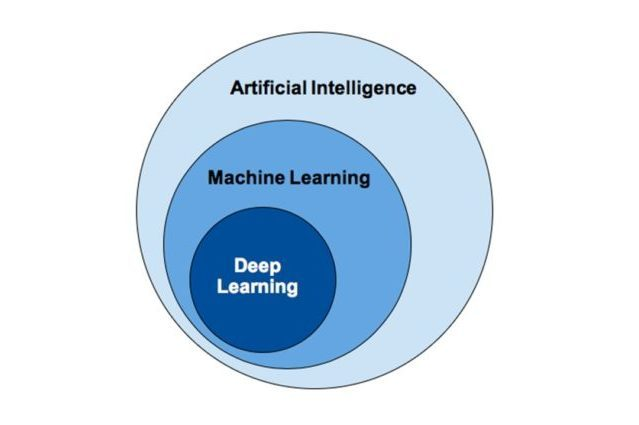
\includegraphics[width=0.6\textwidth]{Images/Chapter1/ai.jpg}
  \caption{Relationship between AI, machine learning, and deep learning.}
  \label{fig:ai}
\end{figure}

\section{Machine Learning}
\label{sec:ml}
Machine learning (\glsxtrshort{ml}) has emerged as a crucial area of study for organizations aiming to harness data resources and gain deeper insights into their operations. Unlike traditional programming methods, where explicit instructions are coded, machine learning enables systems to learn directly from data. In the medical imaging field, ML techniques offer powerful ways to analyze complex MRI data, supporting more accurate and efficient diagnostic processes. However, machine learning is a complex process that involves using diverse algorithms to iteratively learn from data, refine data representations, and make predictions. By feeding training data into these algorithms, increasingly accurate models can be developed. These machine learning models represent the knowledge acquired by algorithms during the training phase \cite{hurwitz2018mlfd}.

\begin{figure}[H]
  \centering
  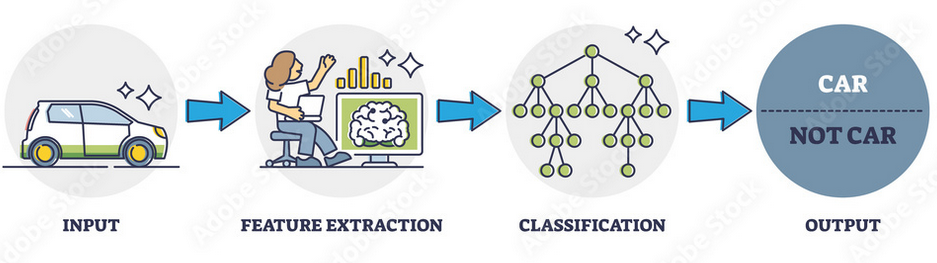
\includegraphics[width=0.8\textwidth]{Images/Chapter1/ml.png}
  \caption{Machine learning process.}
  \label{fig:ml}
\end{figure}
\subsection{Machine Learning approachs}
\subsubsection{Supervised Learning}
In supervised learning, the algorithm learns from labeled training data, where each data point is associated with a corresponding label or target value as depicted in Figure \ref{fig:superml}. Examples of supervised learning algorithms include linear regression , decision trees , random forests , support vector machines , and neural networks.

\begin{figure}[H]
  \centering
  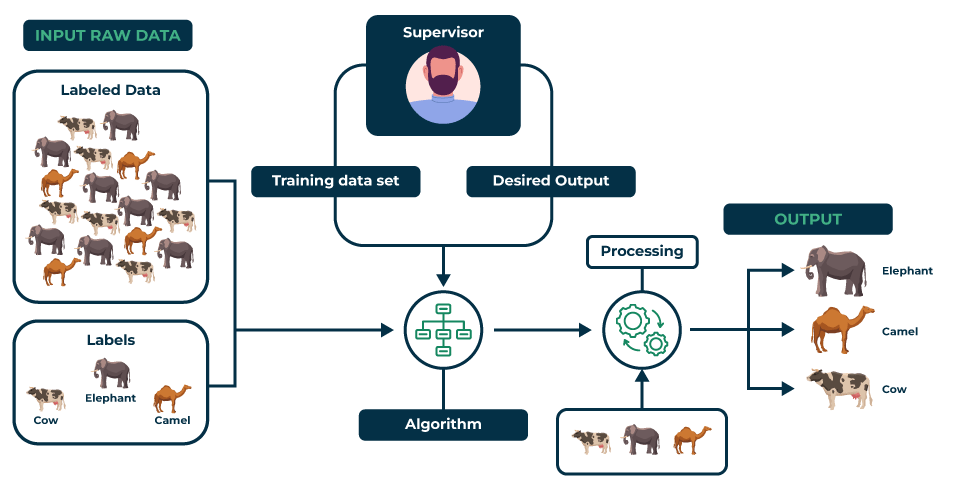
\includegraphics[width=0.8\textwidth]{Images/Chapter1/superml.png}
  \caption{Supervised learning process.}
  \label{fig:superml}
\end{figure}

\subsubsection{Unsupervised Learning}
Unsupervised learning deals with unlabeled data, where the algorithm learns to find patterns or
structure in the data without any specific guidance. Such as k-means and hierarchical
clustering, and dimensionality reduction techniques, such as principal component analysis
and t-distributed stochastic neighbor embedding,  Figure \ref{fig:unsuperml}
\begin{figure}[H]
  \centering
  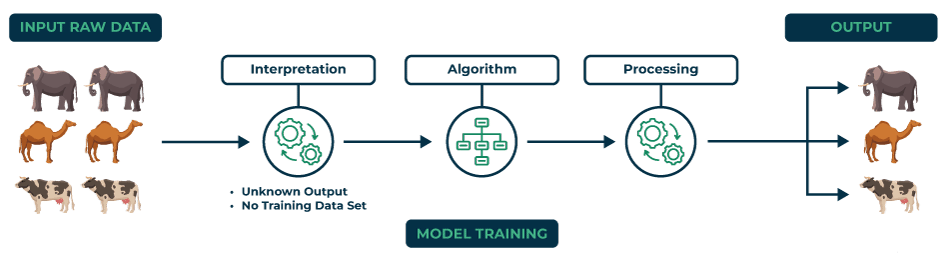
\includegraphics[width=0.8\textwidth]{Images/Chapter1/unsuperml.png}
  \caption{Unsupervised learning process.}
  \label{fig:unsuperml}
\end{figure}

\subsubsection{Reinforcement Learning}
Reinforcement learning is a type of machine learning where an agent learns to make decisions by interacting with an environment. The agent receives feedback in the form of rewards or penalties based on its actions, allowing it to learn optimal strategies over time. This approach is often used in robotics, game playing, and autonomous systems. Figure \ref{fig:reinforcement} illustrates the reinforcement learning process.
\begin{figure}[H]
  \centering
  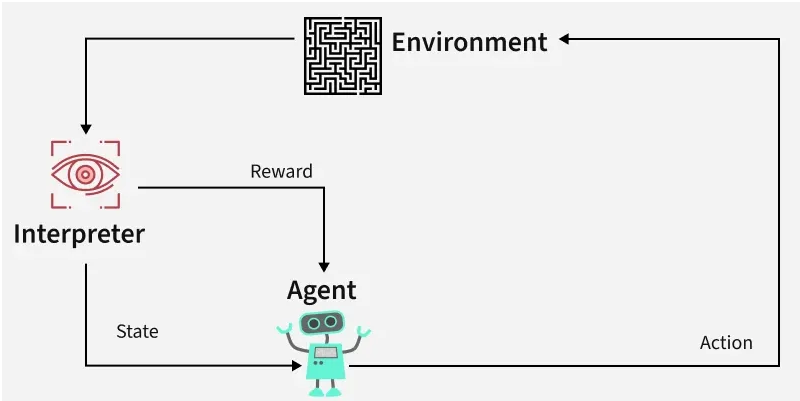
\includegraphics[width=0.8\textwidth]{Images/Chapter1/reinforcement.png}
  \caption{Reinforcement learning process.}
  \label{fig:reinforcement}
\end{figure}

\subsection{Support Vector Machines (SVM)}
\label{sec:svm}
Support Vector Machines (SVMs) are supervised machine learning models widely used for classification and regression tasks. The core idea of SVM is to find an optimal hyperplane that separates data points of different classes with the maximum possible margin, which enhances the model’s ability to generalize to unseen data. SVMs can efficiently handle both linear and non-linear classification problems by employing the kernel trick, which implicitly maps input data into a higher-dimensional feature space where a linear separation becomes possible. The theoretical foundation of SVMs is based on the Structural Risk Minimization (SRM) principle, which aims to minimize an upper bound on the generalization error, offering advantages over traditional Empirical Risk Minimization approaches. Originally developed by Vapnik and colleagues in the 1990s, SVMs have become popular due to their strong empirical performance and robustness to overfitting, especially in high-dimensional spaces \cite{Gunn1998SupportVM}.
\begin{figure}[H]
  \centering
  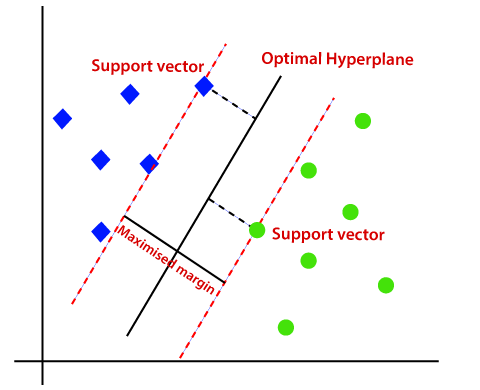
\includegraphics[width=0.4\textwidth]{Images/Chapter1/svm.png}
  \caption{Support Vector Machine.}
  \label{fig:svm}
\end{figure}
The fundamental formula defining the decision boundary of a Support Vector Machine (SVM) is a hyperplane expressed as:
\begin{equation}
  \mathbf{w}^\top \mathbf{x} + b = 0
\end{equation}
where $\mathbf{w}$ is the weight vector normal to the hyperplane, $\mathbf{x}$ is the input feature vector, and $b$ is the bias term.

For binary classification with labels $y_i \in \{+1, -1\}$, the SVM enforces the following constraints on each training point $(\mathbf{x}_i, y_i)$:
\begin{equation}
  y_i \bigl(\mathbf{w}^\top \mathbf{x}_i + b\bigr) \;\ge\; 1,
  \quad \forall\,i.
\end{equation}

The margin width (the distance between the closest points of each class to the hyperplane) is given by $\tfrac{2}{\|\mathbf{w}\|_2}$.  Maximizing this margin is therefore equivalent to minimizing $\|\mathbf{w}\|_2$, leading to the following convex optimization problem:

\begin{align}
  \min_{\mathbf{w},\,b} \quad & \frac{1}{2} \|\mathbf{w}\|_2^2,                             \\
  \text{subject to} \quad     & y_i \bigl(\mathbf{w}^\top \mathbf{x}_i + b\bigr) \;\ge\; 1,
  \quad \forall\,i.
\end{align}

For non-linearly separable data, slack variables and kernel functions can be introduced, but the core formulation remains centered on maximizing the margin around this hyperplane.

\section{Deep Learning}
\label{sec:dl}
Deep learning has emerged as a powerful approach for modeling complex data through intricate architectures that incorporate non-linear transformations. Neural networks, including deep neural networks, serve as the fundamental components of deep learning. These techniques have achieved remarkable progress in various domains such as sound and image processing, enabling tasks like facial recognition, speech recognition, computer vision, language processing, and text classification. The potential applications of deep learning are vast and continue to expand.

Different types of neural network architectures, such as multilayer perceptrons, Convolutional Neural Networks (\glsxtrshort{cnn}s), and recurrent neural networks, cater to specific data types and tasks. These architectures are characterized by deep layers organized in a cascading manner. Successful implementation of deep learning requires well-designed stochastic optimization algorithms, appropriate initialization techniques, and thoughtful structure selection.

\begin{figure}[H]
  \centering
  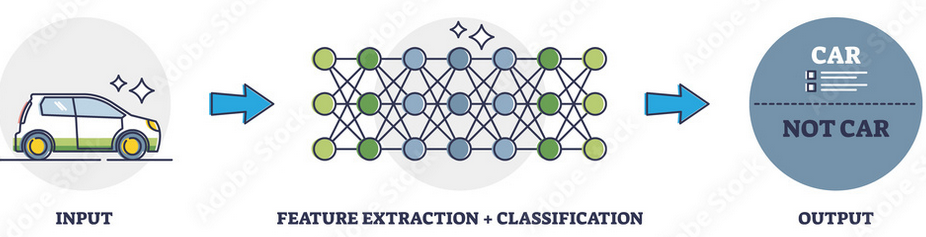
\includegraphics[width=0.8\textwidth]{Images/Chapter1/dl.png}
  \caption{Deep learning process.}
  \label{fig:dl}
\end{figure}

\subsection{Convolutional Neural Networks (CNNs)}
\label{sec:cnn}
A convolutional neural network (CNN) is a type of neural network with a topology similar to a grid, inspired by the human brain. It is commonly used for image processing tasks, as well as natural language processing.

A CNN consists of two main parts. The input is an image, represented as a 2D matrix of pixels for grayscale images and a 3D matrix of pixels for color images (Red, Green, Blue).

The first part of a CNN is the convolutional layer, which acts as a feature extractor. The image is passed through a series of filters, or convolution kernels, to generate new images called feature maps. Some intermediate filters reduce the image resolution. Finally, the feature maps are concatenated to form a vector of features, known as the CNN code.

The output of the convolutional layer, the CNN code, is the input to the second part of the network. The main role of this part is to combine the features of the CNN code to classify the image. The output is a final layer with one neuron per category.
\begin{figure}[H]
  \centering
  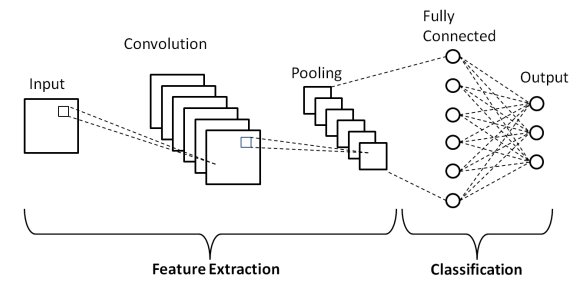
\includegraphics[width=0.8\textwidth]{Images/Chapter1/cnn.png}
  \caption{Convolutional Neural Network.}
  \label{fig:cnn}
\end{figure}

\subsubsection{Convolutional Layer}
\label{sec:conv}

The convolutional layer is the most important layer and usually the first layer in a CNN. It consists of three main elements involved in the convolution operation:
\begin{itemize}
  \item \textbf{Input image} ($f$)
  \item \textbf{Feature detector (filter)} ($h$)
  \item \textbf{Feature map (output)} ($G$)
\end{itemize}

A convolution takes an image and a filter as input and applies the convolution operation to produce a new image, called the activation map or feature map.

The activation map values are calculated using the following formula:
\begin{equation}
  G[m,n] \;=\; (f * h)[m,n]
\end{equation}
where
\begin{itemize}
  \item $f$ is the input image,
  \item $h$ is the convolution filter,
  \item $m,n$ are the spatial indices over which the convolution is computed.

\end{itemize}
\begin{figure}[H]
  \centering
  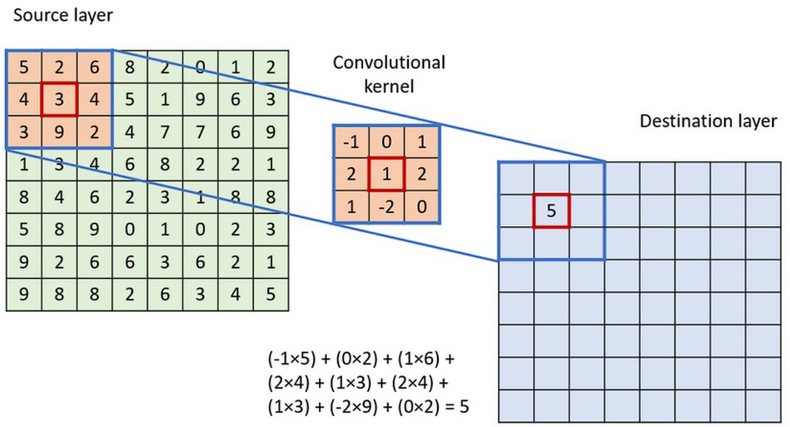
\includegraphics[width=0.6\textwidth]{Images/Chapter1/conv.png}
  \caption{Convolution Layer.}
  \label{fig:conv}
\end{figure}

\subsubsection{Correction Layer (ReLU)}

The Correction Layer, typically implemented using the Rectified Linear Unit (ReLU), is an activation function applied after each convolution operation to enhance processing efficiency. It replaces all negative pixel values with zero, introducing non-linearity into the network while maintaining computational simplicity. The ReLU function is defined as:

\begin{equation}
  f(x) = \max(0, x)
\end{equation}

Several other activation functions exist, such as the sigmoid function, the hyperbolic tangent function (tanh), and the hyperbolic saturating tangent function. However, ReLU is often preferred in deep learning models because it enables faster convergence and better performance compared to these alternatives.

\subsubsection{Pooling Layers}

Pooling layers are utilized to reduce the spatial dimensions of feature maps while preserving the most important information and features. This helps decrease computational complexity and mitigate overfitting. There are several types of pooling operations:

\begin{itemize}
  \item \textbf{Max Pooling}:
        It selects the maximum value from each patch of the feature map. Typically, a $2 \times 2$ patch is used. Max pooling is the most commonly used pooling method.

  \item \textbf{Min Pooling}:
        The inverse of max pooling; it selects the minimum value from each patch of the feature map.

  \item \textbf{Average Pooling}:
        It computes the average of all the values within each patch of the feature map by summing the values and dividing by the number of elements.

  \item \textbf{Sum Pooling}:
        It computes the sum of all elements within each patch of the feature map.

  \item \textbf{Flattening}:
        After the pooling operations, the resulting feature maps are flattened into a single one-dimensional vector to prepare for fully connected (dense) layers.
\end{itemize}

\subsubsection{Fully Connected Layer}

after the convolution and pooling layers, the high-level reasoning in the neural network is done in fully connected layers. The output of flattening is the input of FC layers which are the same as artificial neural networks and carry out the same mathematical operations. The last fully-connected layer uses an activation function such as sigmoid or softmax to get probabilities of the outputs.

\subsection{U-Net Architecture}
U-Net is a convolutional neural network architecture specifically designed for biomedical image segmentation. Introduced by Ronneberger et al. in 2015, U-Net features a symmetric encoder-decoder structure: the contracting path (encoder) captures image context through successive convolution and pooling operations, while the expansive path (decoder) enables precise localization via upsampling and concatenation with high-resolution features from the encoder. This architecture allows U-Net to achieve accurate segmentation even with limited annotated data by leveraging extensive data augmentation. U-Net has demonstrated superior performance in various biomedical segmentation challenges, notably outperforming previous methods in tasks such as neuronal structure segmentation in electron microscopy images and cell tracking in light microscopy \cite{ronneberger2015u}.

\begin{figure}[H]
  \centering
  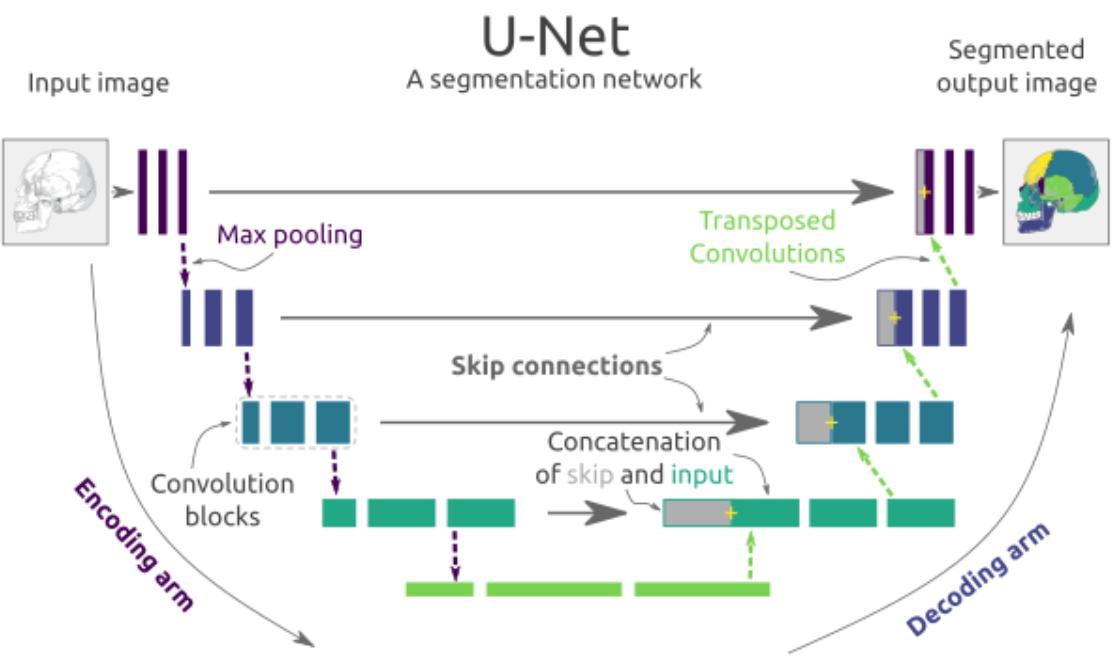
\includegraphics[width=0.8\textwidth]{Images/Chapter1/unet2.png}
  \caption{U-Net Architecture.}
  \label{fig:unet}
\end{figure}

\subsubsection{Key Components of a U-Net Architecture}

\begin{itemize}
  \item \textbf{Contracting Path (Encoder):} \\
        This path is responsible for extracting contextual features from the input image. It consists of repeated blocks of two $3\times3$ convolutional layers (with ReLU activation), followed by a $2\times2$ max pooling operation for downsampling. With each downsampling step, the number of feature channels is doubled, allowing the network to capture increasingly abstract representations of the input.

  \item \textbf{Bottleneck:} \\
        Located at the deepest part of the network, the bottleneck consists of convolutional layers without pooling. It serves as the bridge between the encoder and decoder, capturing the most condensed and abstract features of the input.

  \item \textbf{Expansive Path (Decoder):} \\
        This path reconstructs the spatial resolution of the feature maps and enables precise localization. Each step in the decoder involves upsampling the feature map (often via transposed convolution or up-convolution), concatenating it with the corresponding feature map from the encoder (skip connection), and then applying two $3\times3$ convolutions (with ReLU activation). The number of feature channels is halved at each upsampling step.

  \item \textbf{Skip Connections:} \\
        At each level, feature maps from the encoder are concatenated with the upsampled feature maps in the decoder. These skip connections help retain high-resolution spatial information that might otherwise be lost during downsampling, improving the accuracy of segmentation boundaries.

  \item \textbf{Final Output Layer:} \\
        The last layer is typically a $1\times1$ convolution that maps each feature vector to the desired number of output classes, producing a pixel-wise classification map for segmentation tasks.
\end{itemize}

This U-shaped design enables U-Net to effectively combine global context with fine-grained localization, making it highly effective for precise image segmentation tasks.

\subsection{Megnatic Resonance Imaging (MRI)}
\label{sec:mri}
Magnetic resonance imaging (MRI) uses a powerful magnetic field and radio waves to
generate detailed and high-resolution images of organs and tissues inside the human body, as
depicted in Figure \ref{fig:mri}. This non-invasive imaging method offers significant advantages in
visualizing intricate details of the brain, spinal cord, joints, and soft tissues. MRI plays a vital
role in diagnosing and evaluating a wide range of medical conditions, such as tumors,
neurological disorders, and musculoskeletal injuries. Its ability to produce precise and detailed
images aids healthcare professionals in accurately identifying and assessing these conditions,
enabling effective treatment planning and optimal patient care \cite{verywell_mri}.

\begin{figure}[H]
  \centering
  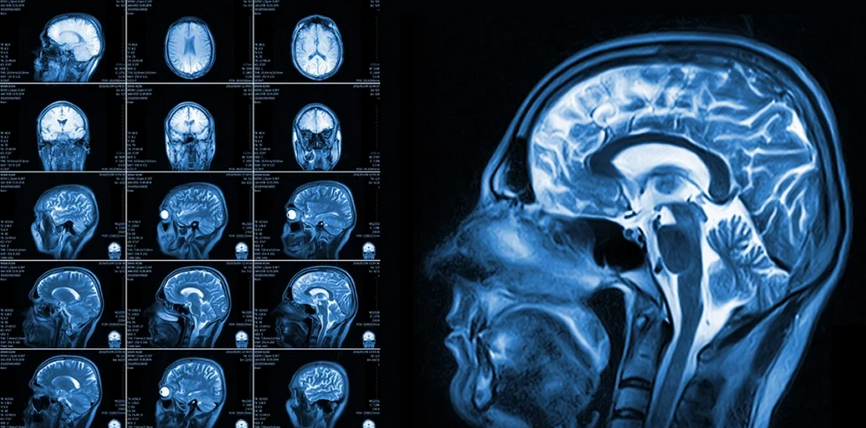
\includegraphics[width=0.6\textwidth]{Images/Chapter1/mri.png}
  \caption{Magnetic Resonance Imaging (MRI).}
  \label{fig:mri}
\end{figure}

\section{Conclusion}
\label{sec:conclusion}

In this chapter, we established the theoretical foundation necessary for our study on brain tumor analysis using artificial intelligence techniques. We first explored the fundamental concepts of artificial intelligence, machine learning, and deep learning, emphasizing their significance in the medical imaging domain. We discussed the various machine learning approaches, highlighting the principles and applications of Support Vector Machines (SVMs) for classification tasks. Furthermore, we introduced deep learning methodologies, focusing on Convolutional Neural Networks (CNNs) and their components, including convolutional, pooling, and fully connected layers. Finally, we presented the U-Net architecture, a specialized CNN model for biomedical image segmentation, which plays a crucial role in the segmentation phase of our proposed hybrid approach. This theoretical background sets the stage for the practical implementation and evaluation of our models in the following chapters.

\chapter{State of the Art}

\section{Medical Imaging in Brain Tumor Diagnosis}

Magnetic Resonance Imaging (MRI) has emerged as the gold standard for brain tumor diagnosis due to its superior soft tissue contrast, high spatial resolution, and non-invasive nature \cite{Bauer2013}. Unlike other imaging modalities such as CT scans, MRI provides detailed structural information without exposing patients to ionizing radiation, making it particularly valuable for serial monitoring and treatment planning \cite{Menze2015}.

The multimodal nature of MRI is especially useful in brain tumor assessment, with each sequence highlighting different aspects of the tumor \cite{Bakas2018}:

\begin{itemize}
  \item \textbf{T1-weighted (T1)}: Provides excellent anatomical detail and clearly delineates boundaries between gray and white matter. Tumors typically appear hypointense (darker) compared to surrounding tissue.

        \begin{minipage}{\linewidth}
          \centering
          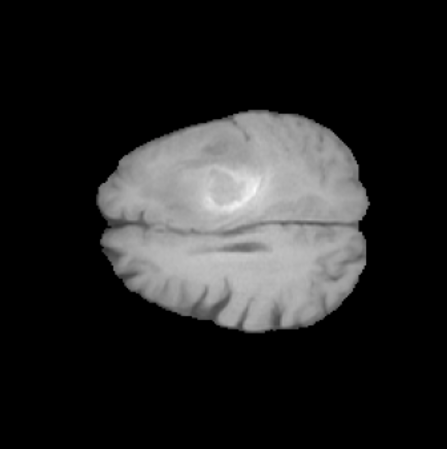
\includegraphics[width=0.4\textwidth]{./Images/Chapter2/t1.png}
          \captionsetup{hypcap=false}
          \captionof{figure}{Example of T1-weighted MRI sequence.}
          \label{fig:t1}
        \end{minipage}
        \vspace{\baselineskip}

  \item \textbf{T1 with contrast enhancement (T1ce)}: After gadolinium administration, areas with disrupted blood-brain barrier (characteristic of high-grade tumors) enhance, appearing hyperintense and revealing the active tumor core.

        \begin{minipage}{\linewidth}
          \centering
          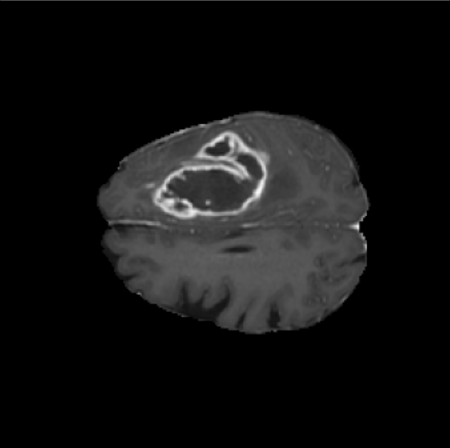
\includegraphics[width=0.4\textwidth]{./Images/Chapter2/t1ce.png}
          \captionsetup{hypcap=false}
          \captionof{figure}{Example of T1-weighted contrast-enhanced MRI sequence.}
          \label{fig:t1ce}
        \end{minipage}
        \vspace{\baselineskip}

  \item \textbf{T2-weighted (T2)}: Highlights areas with increased water content, making it valuable for identifying edema and infiltrative tumor components. Tumors and surrounding edema appear hyperintense.

        \begin{minipage}{\linewidth}
          \centering
          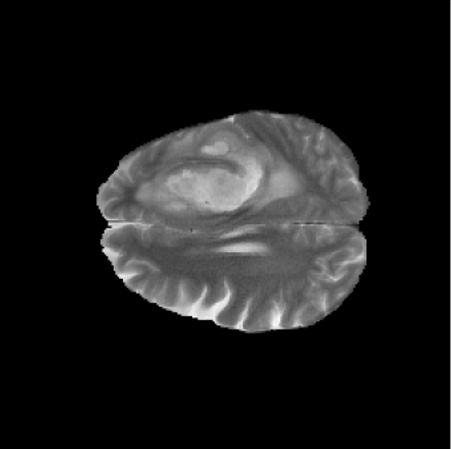
\includegraphics[width=0.4\textwidth]{./Images/Chapter2/t2.png}
          \captionsetup{hypcap=false}
          \captionof{figure}{Example of T2-weighted MRI sequence.}
          \label{fig:t2}
        \end{minipage}
        \vspace{\baselineskip}

  \item \textbf{Fluid-Attenuated Inversion Recovery (FLAIR)}: Suppresses cerebrospinal fluid signals, enhancing the visibility of periventricular lesions and edema associated with tumors.

        \begin{minipage}{\linewidth}
          \centering
          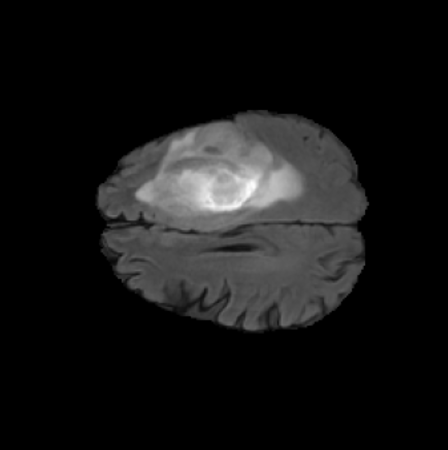
\includegraphics[width=0.4\textwidth]{./Images/Chapter2/flair.png}
          \captionsetup{hypcap=false}
          \captionof{figure}{Example of FLAIR MRI sequence.}
          \label{fig:t2-flair}
        \end{minipage}
        \vspace{\baselineskip}
\end{itemize}


Traditionally, neuroradiologists diagnose brain tumors by visually inspecting these multiple MRI sequences, mentally integrating information across modalities to determine tumor boundaries, assess grade, and identify critical structures \cite{DeAngelis2001}. This process is inherently subjective, time-consuming, and susceptible to inter-observer variability, with studies reporting considerable disagreement even among experienced radiologists  These limitations have driven significant interest in developing computational approaches for automated and semi-automated tumor analysis.

\section{The BraTS Dataset}

The Brain Tumor Segmentation (BraTS) challenge and dataset represent a landmark initiative in standardizing the evaluation of brain tumor segmentation algorithms \cite{Menze2015, Bakas2018}. Since its inception in 2012, BraTS has evolved into the most widely adopted benchmark for algorithm development and performance assessment in this domain \cite{Bakas2019}.

The BraTS dataset is particularly valuable due to its:

\begin{itemize}
  \item \textbf{Multimodal approach}: Each case includes four co-registered MRI sequences (T1, T1ce, T2, and FLAIR), enabling algorithms to leverage complementary information \cite{Bakas2017}.
  \item \textbf{Standardized preprocessing}: All images undergo skull-stripping, resampling to isotropic 1mm³ voxels, and registration to a common anatomical template, reducing technical variability \cite{Bakas2018}.
  \item \textbf{Expert annotations}: Each tumor is manually segmented by experienced neuroradiologists following a standardized protocol, with additional verification to ensure quality \cite{Menze2015}.
  \item \textbf{Multi-institutional data}: Images are acquired from multiple institutions using different scanners and protocols, promoting the development of robust algorithms \cite{Bakas2019}.
\end{itemize}

\begin{enumerate}
  \item \textbf{Enhancing Tumor (ET)}: Areas showing hyperintensity in T1ce relative to T1
  \item \textbf{Tumor Core (TC)}: Encompassing the ET, necrotic components, and non-enhancing tumor
  \item \textbf{Whole Tumor (WT)}: Including all tumor tissues and surrounding edema
\end{enumerate}

This hierarchical annotation structure enables the evaluation of algorithms at multiple levels of detail, from gross tumor detection to fine-grained sub-region delineation \cite{Bakas2018}. The BraTS datasets and associated challenges have catalyzed significant methodological advances, with performance metrics improving consistently year over year \cite{Isensee2021}.

\section{Traditional Machine Learning Approaches}

Before the deep learning revolution, brain tumor segmentation and classification relied heavily on traditional machine learning techniques coupled with handcrafted feature extraction \cite{Gordillo2013}. These approaches typically followed a pipeline of preprocessing, feature extraction, and classification using conventional machine learning algorithms.

\textbf{Support Vector Machines (\glsxtrshort{svm})} were particularly popular for brain tumor classification and segmentation due to their strong theoretical foundations and effectiveness with high-dimensional data \cite{Bauer2011}. Zacharaki et al.\ \cite{Zacharaki2009} developed an \glsxtrshort{svm}-based system that extracted 161 features including intensity, texture, and shape characteristics from multi-parametric \glsxtrshort{mri}, achieving 85\% accuracy in discriminating between different tumor types. Similarly, Reza and Iftekharuddin \cite{Reza2013} combined texture features with fractal analysis and \glsxtrshort{svm} classification to segment brain tumors, demonstrating competitive performance on earlier \glsxtrshort{brats} datasets.

\textbf{Random Forest (\glsxtrshort{rf})} classifiers also showed promise due to their robustness to overfitting and ability to handle multi-class problems efficiently. Zikic et al.\ \cite{Zikic2012} employed \glsxtrshort{rf} with context-aware features for brain tumor segmentation, while Festa et al.\ \cite{Festa2013} achieved strong results in the BraTS 2013 challenge using RF with handcrafted features. Tustison et al.\ \cite{Tustison2015} further refined this approach by incorporating an extensive feature set derived from multiple MRI sequences, winning the BraTS 2013 challenge.

\textbf{K-Nearest Neighbors (\glsxtrshort{knn})} algorithms were explored by Simi and Joseph \cite{Simi2014}, who combined texture features with k-NN classification for tumor segmentation. Huang et al.\ \cite{Huang2014} also investigated k-NN for brain tumor classification using multispectral MRI features.

Despite their success, these traditional approaches faced significant limitations:

\begin{itemize}
  \item \textbf{Dependence on handcrafted features}: Their performance was heavily contingent on the quality of manually designed features, requiring substantial domain expertise \cite{Pandit2019}.
  \item \textbf{Limited contextual understanding}: Most methods struggled to incorporate broader spatial context, often relying on voxel-wise or small-patch features \cite{Havaei2017}.
  \item \textbf{Computational inefficiency}: Sequential processing of feature extraction followed by classification led to lengthy processing times impractical for clinical settings \cite{Sompong2017}.
  \item \textbf{Suboptimal performance on heterogeneous tumors}: The high variability in tumor appearance often challenged these methods, particularly for complex or atypical cases \cite{Menze2015}.
\end{itemize}

These limitations ultimately paved the way for the adoption of deep learning techniques, which could learn hierarchical features directly from data and better capture the complex patterns present in brain tumor images.

\section{Deep Learning in Brain Tumor Segmentation}

The adoption of deep learning, particularly Convolutional Neural Networks (\glsxtrshort{cnn}), has revolutionized brain tumor segmentation by enabling automatic hierarchical feature learning directly from imaging data \cite{Havaei2017}. This paradigm shift has eliminated the need for handcrafted features, and led to improving segmentation accuracy and robustness.

Among deep learning architectures, U-Net has emerged as the cornerstone for medical image segmentation, including brain tumor analysis \cite{Ronneberger2015}. Its distinctive encoder-decoder structure with skip connections effectively combines localization and contextual information, preserving fine details while capturing broader tumor patterns. Urban et al.\ \cite{Urban2014} were among the first to apply CNNs to brain tumor segmentation, while Pereira et al.\ \cite{Pereira2016} demonstrated that carefully designed CNN architectures could outperform traditional methods on the BraTS challenge.

Several U-Net variants have been developed specifically for brain tumor segmentation:

\begin{itemize}
  \item \textbf{3D U-Net}: Çiçek et al.\ \cite{Cicek2016} extended the original 2D architecture to process volumetric data, better capturing the three-dimensional nature of tumors. Isensee et al.\ \cite{Isensee2018} further refined this approach, achieving top ranking in the BraTS 2018 challenge with a 3D U-Net variant.

  \item \textbf{U-Net++}: Zhou et al.\ \cite{Zhou2019} proposed a nested architecture with redesigned skip pathways to bridge the semantic gap between encoder and decoder features. Experimental results showed improved performance on several medical segmentation tasks, including brain tumors.

  \item \textbf{Attention U-Net}: Oktay et al.\ \cite{Oktay2018} incorporated attention gates to highlight relevant features and suppress irrelevant regions, improving segmentation accuracy particularly at tumor boundaries. Schlemper et al.\ \cite{Schlemper2019} demonstrated the effectiveness of this approach for multi-class tumor segmentation.
\end{itemize}

The performance of these deep learning models on BraTS challenges has improved consistently over time. In BraTS 2018, Myronenko \cite{Myronenko2018} achieved exceptional results with an encoder-decoder architecture incorporating variational components. McKinley et al.\ \cite{McKinley2019} further advanced the field with an ensemble of 3D U-Nets, achieving Dice scores of 0.91, 0.83, and 0.78 for whole tumor, tumor core, and enhancing tumor, respectively. The BraTS 2020 challenge saw even more impressive results, with top-performing methods consistently achieving Dice scores above 0.90 for whole tumor segmentation \cite{Isensee2021}.

Despite these advancements, challenges remain in achieving clinically acceptable performance across diverse patient populations and imaging protocols, driving continuous innovation in the field.

\section{Tumor Classification Using Deep Features}

While segmentation delineates tumor boundaries, classification determines tumor type and characteristics—a critical aspect of diagnosis and treatment planning. Modern approaches increasingly leverage deep features, either independently or in conjunction with traditional machine learning classifiers like Support Vector Machines (SVMs).

Pretrained Convolutional Neural Networks (CNNs) have proven extremely effective as feature extractors for brain tumor classification. Afshar et al.\ \cite{Afshar2019} employed a modified ResNet architecture to extract deep features from brain MRI, achieving 93.68\% accuracy in classifying tumors into different grades. Similarly, Deepak and Ameer \cite{Deepak2019} utilized DenseNet for feature extraction followed by SVM classification, reporting improved performance compared to traditional methods. Sajjad et al.\ \cite{Sajjad2019} extended this approach by fine-tuning VGG-19 on brain tumor images, extracting features from intermediate layers for subsequent classification.

\section{Multiclass Tumor Region Segmentation}

Accurate delineation of different tumor sub-regions represents one of the most challenging aspects of brain tumor analysis, requiring discrimination between biologically distinct components that may appear visually similar \cite{Bakas2018}. The BraTS challenge specifically evaluates algorithms on their ability to segment three tumor sub-components: Enhancing Tumor (ET), Tumor Core (TC), and Whole Tumor (WT).

Multi-class tumor segmentation approaches have evolved significantly in recent years. Zhao et al.\ \cite{Zhao2018} proposed a multi-scale CNN architecture specifically designed to address the hierarchical nature of tumor sub-regions, achieving meaningful improvements in enhancing tumor segmentation. Wang et al.\ \cite{Wang2017} developed a cascaded approach where initial whole tumor segmentation guided subsequent sub-region delineation, reducing false positives in non-tumor regions. Kamnitsas et al.\ \cite{Kamnitsas2017} introduced DeepMedic, a dual-pathway 3D CNN architecture that simultaneously processed input at different resolutions, effectively capturing both fine details and broader contextual information.

The continued advancement of multi-class tumor segmentation approaches promises to improve diagnostic accuracy and treatment planning by providing more detailed characterization of tumor heterogeneity.

\section{Challenges in the Field}

Despite the significant progress, several persistent challenges continue to impact the development and clinical translation of automated brain tumor analysis systems.

\textbf{Class imbalance} remains a fundamental issue in both segmentation and classification tasks. Brain tumors typically occupy less than 1\% of the total brain volume, creating extreme imbalance that can bias models toward the majority (healthy tissue) class \cite{Pereira2016}. While techniques such as patch-based training \cite{Havaei2017}, specialized loss functions \cite{Isensee2018}, and data augmentation \cite{Wang2019} have partially addressed this issue, performance on smaller tumor sub-regions (particularly enhancing tumor) continues to lag behind whole tumor segmentation.

The \textbf{interpretability of deep models} presents another significant hurdle, particularly for clinical adoption. The "black box" nature of deep learning approaches creates reluctance among clinicians to trust automated segmentations without understanding the underlying decision process \cite{Holzinger2017}. Recent work by Natekar et al.\ \cite{Natekar2020} has explored visualization techniques to highlight features influencing segmentation decisions, while Lucieri et al.\ \cite{Lucieri2020} demonstrated the value of attention maps for explaining tumor classification outcomes. However, creating truly interpretable deep learning systems remains an open challenge.

\textbf{Generalization across different MRI scanners and patients} continues to limit clinical applicability. Models trained on specific datasets often experience performance degradation when applied to images acquired with different hardware, field strengths, or acquisition parameters \cite{Menze2015}. Zech et al.\ \cite{Zech2018} documented this domain shift problem in medical imaging, while Kamnitsas et al.\ \cite{Kamnitsas2017} proposed domain adaptation techniques to mitigate its effects. More recently, Shaw et al.\ \cite{Shaw2020} explored adversarial domain adaptation specifically for brain tumor segmentation, showing promising results in cross-scanner generalization.

The \textbf{lack of labeled data} remains a fundamental limitation, particularly for rare tumor types or unusual presentations. While the BraTS dataset has grown substantially, it still represents a fraction of the true biological variability of brain tumors \cite{Bakas2019}. Semi-supervised approaches by Sedai et al.\ \cite{Sedai2019} leverage unlabeled data to improve generalization, while Zhao et al.\ \cite{Zhao2019b} demonstrated promising results with data-efficient few-shot learning techniques. Transfer learning approaches by Ghafoorian et al.\ \cite{Ghafoorian2017} have also shown potential in adapting pre-trained models to limited target datasets.

Additional challenges include:

\begin{itemize}
  \item \textbf{Computational efficiency}: 3D deep learning models often require substantial computational resources beyond what's available in many clinical settings \cite{Kamnitsas2017}.
  \item \textbf{Longitudinal analysis}: Most current approaches treat each time point independently, missing the opportunity to leverage temporal information in patient monitoring \cite{Weninger2018}.
  \item \textbf{Integration with other data types}: Combining imaging with clinical, genomic, and pathological data remains challenging despite its potential to improve diagnostic accuracy \cite{Bakas2019}.
  \item \textbf{Clinically relevant evaluation metrics}: Standard technical metrics like Dice coefficients may not directly translate to clinical utility, creating a disconnect between research advances and clinical impact \cite{MaierHein2018}.
\end{itemize}

Addressing these challenges will require multidisciplinary collaboration between computer scientists, medical imaging experts, and clinicians to develop solutions that are not only technically sophisticated but also clinically relevant and practically deployable.

\chapter{Contribution}

\section{Introduction}
\label{sec:contribution-introduction}

In this chapter, we present the core contributions of our work on automated brain tumor detection in MRIs. Building upon the BraTS dataset \cite{Menze2015}, our pipeline integrates a deep learning–based segmentation module with a classical machine learning classifier and culminates in a user‐friendly demo application.

\section{Proposed Framework Overview}
\label{sec:contribution-framework}
In this section, we look at our proposed fremework from a systematic perspective. The framework is designed to perform end-to-end brain tumor segmentation and classification. We will discuss the design of the final pipeline and the training workflow to achieve the desired results.

\subsection{End-to-End Inference Pipeline}
The purpose of our project is to have an end-to-end inference pipeline accepts a raw MR image as input, applies preprocessing steps, performs segmentation of the tumor region using the trained U-Net model, classifies the tumor grade via the SVM classifier, and finally outputs the original image overlaid with the segmentation mask along with the predicted grade as shown in Figure~\ref{fig:pipeline}.
\begin{figure}[H]
  \centering
  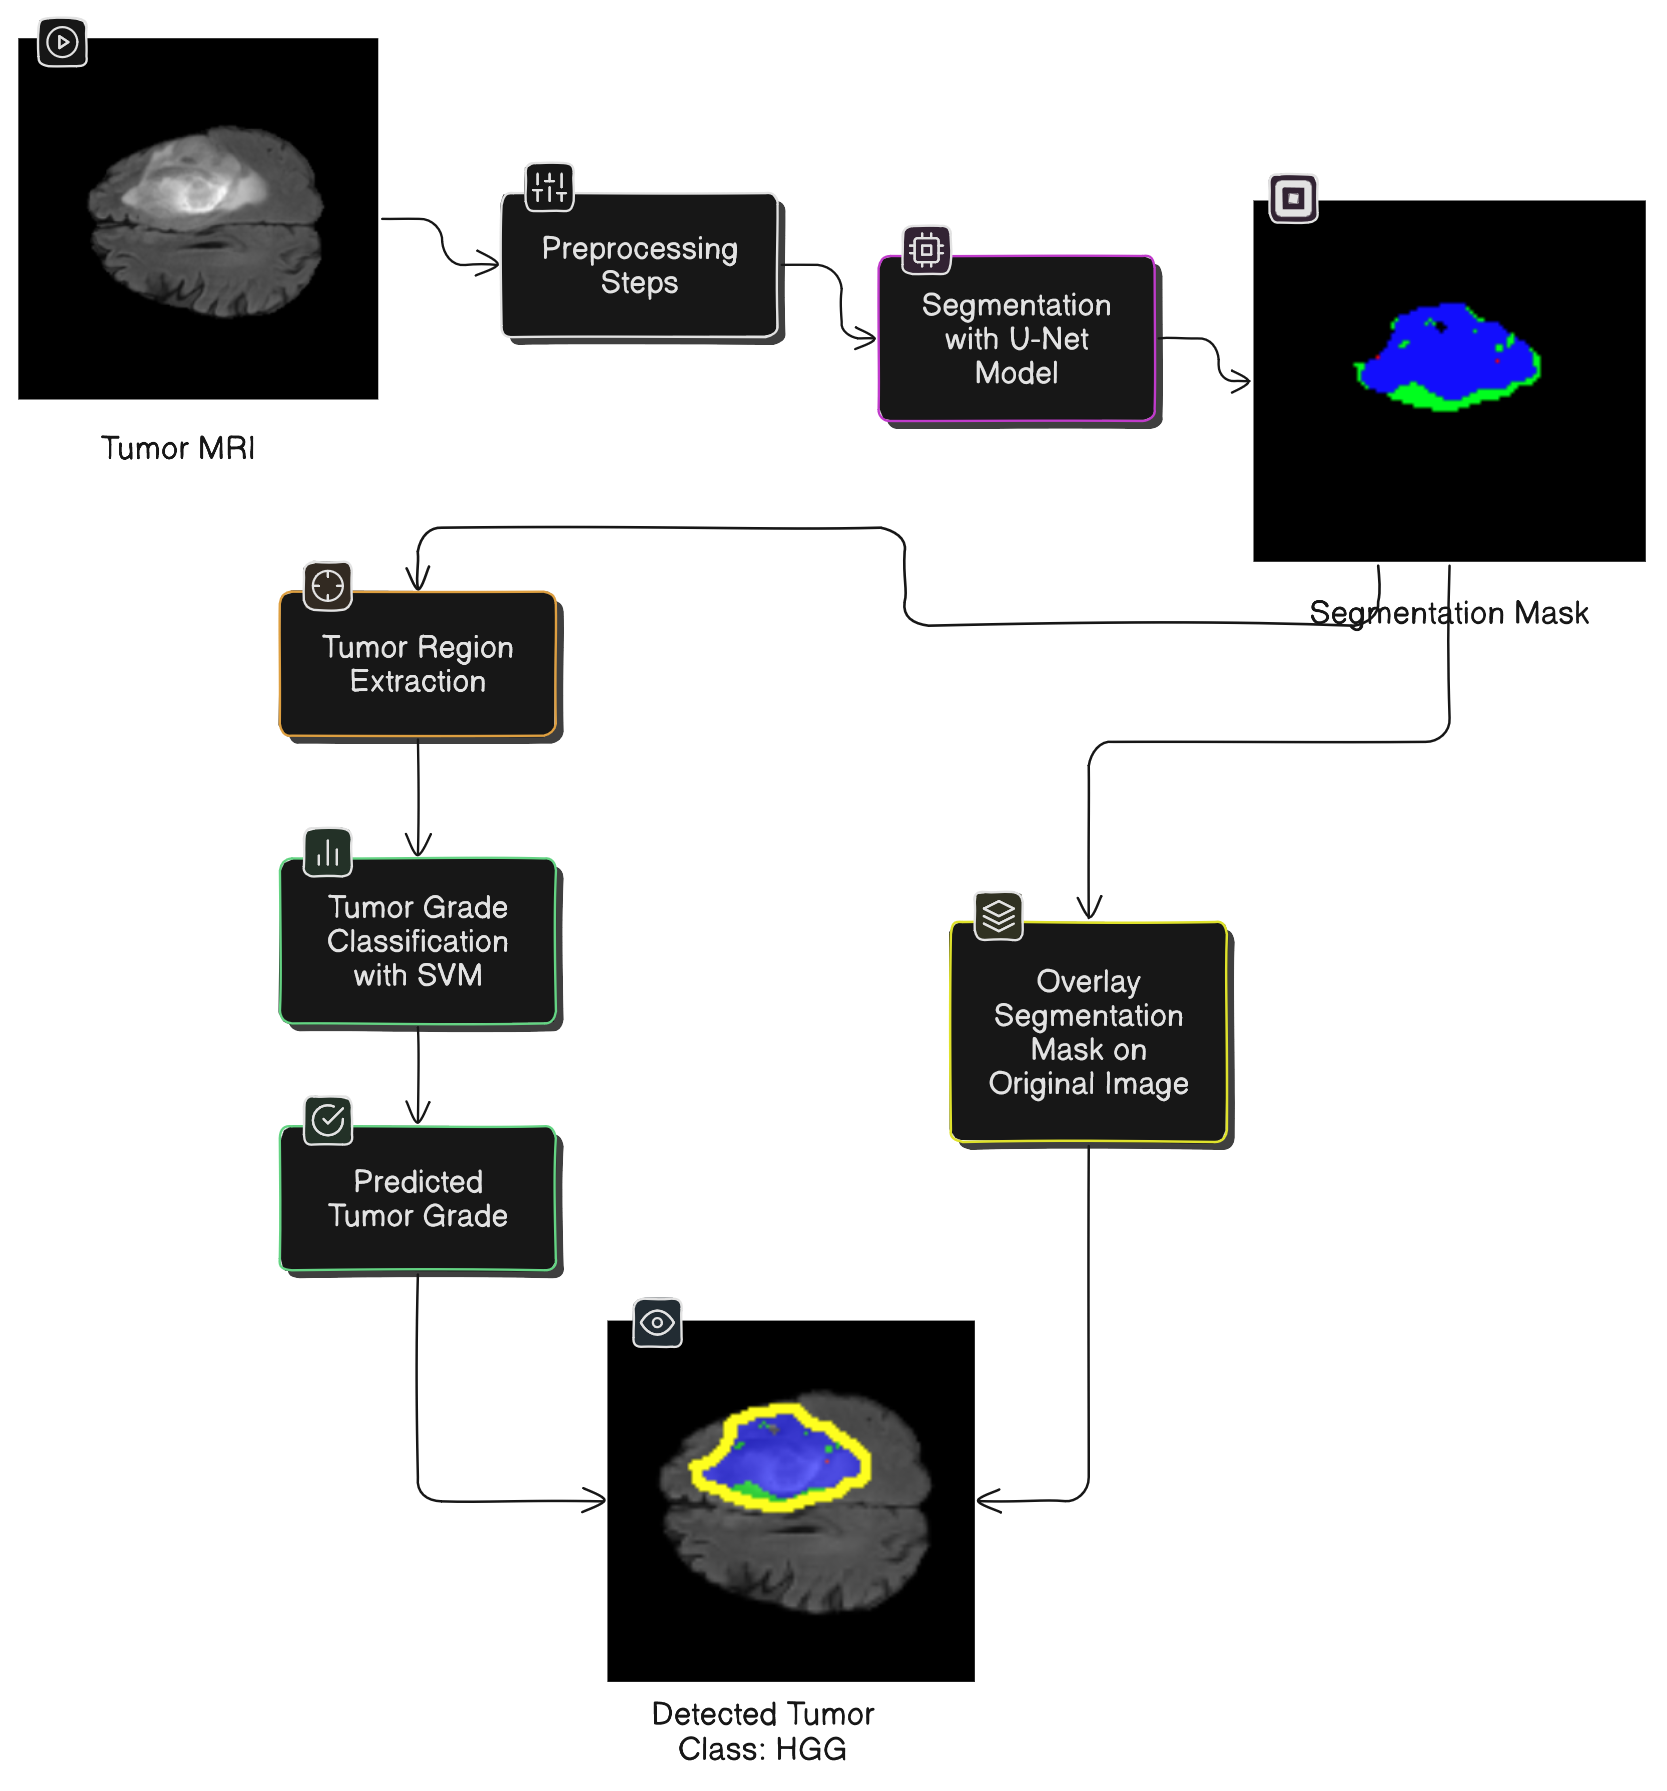
\includegraphics[width=0.8\textwidth]{Images/Chapter3/pipeline.png}
  \caption{Overview of the end-to-end inference pipeline.}
  \label{fig:pipeline}
\end{figure}
The selection of U-Net for tumor segmentation and Support Vector Machine (SVM) for tumor grade classification in our end-to-end inference pipeline is grounded in their proven efficacy in medical image analysis, particularly in brain tumor applications.

\subsubsection{U-Net for Tumor Segmentation}
U-Net is a convolutional neural network architecture specifically designed for biomedical image segmentation. Its encoder-decoder structure with skip connections allows for precise localization and context capture, making it highly effective for segmenting complex structures like brain tumors. Studies have demonstrated that U-Net and its variants achieve high accuracy in delineating tumor boundaries in MRI images, even with limited training data \cite{dong2017automatic, walsh2022using}.

Introduced by Ronneberger et al. in 2015, U-Net features a symmetric encoder-decoder structure: the contracting path (encoder) captures image context through successive convolution and pooling operations, while the expansive path (decoder) enables precise localization via upsampling and concatenation with high-resolution features from the encoder. This architecture allows U-Net to achieve accurate segmentation even with limited annotated data by leveraging extensive data augmentation. U-Net has demonstrated superior performance in various biomedical segmentation challenges, notably outperforming previous methods in tasks such as neuronal structure segmentation in electron microscopy images and cell tracking in light microscopy \cite{ronneberger2015u}.
\begin{figure}[H]
  \centering
  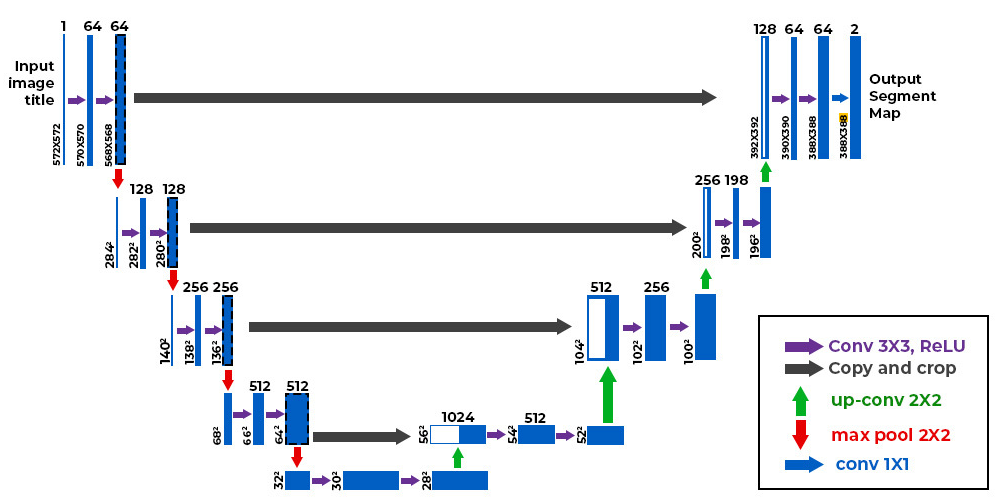
\includegraphics[width=0.8\textwidth]{Images/Chapter1/unet.png}
  \caption{U-Net Architecture Illustrating the Encoding and Decoding Arms with Skip Connections. \cite{ronneberger2015u}}
  \label{fig:unet}
\end{figure}

\paragraph*{Key Components of a U-Net Architecture}

\begin{itemize}
  \item \textbf{Contracting Path (Encoder):} \\
        This path is responsible for extracting contextual features from the input image. It consists of repeated blocks of two $3\times3$ convolutional layers (with ReLU activation), followed by a $2\times2$ max pooling operation for downsampling. With each downsampling step, the number of feature channels is doubled, allowing the network to capture increasingly abstract representations of the input.

  \item \textbf{Bottleneck:} \\
        Located at the deepest part of the network, the bottleneck consists of convolutional layers without pooling. It serves as the bridge between the encoder and decoder, capturing the most condensed and abstract features of the input.

  \item \textbf{Expansive Path (Decoder):} \\
        This path reconstructs the spatial resolution of the feature maps and enables precise localization. Each step in the decoder involves upsampling the feature map (often via transposed convolution or up-convolution), concatenating it with the corresponding feature map from the encoder (skip connection), and then applying two $3\times3$ convolutions (with ReLU activation). The number of feature channels is halved at each upsampling step.

  \item \textbf{Skip Connections:} \\
        At each level, feature maps from the encoder are concatenated with the upsampled feature maps in the decoder. These skip connections help retain high-resolution spatial information that might otherwise be lost during downsampling, improving the accuracy of segmentation boundaries.

  \item \textbf{Final Output Layer:} \\
        The last layer is typically a $1\times1$ convolution that maps each feature vector to the desired number of output classes, producing a pixel-wise classification map for segmentation tasks.
\end{itemize}

\subsubsection{SVM for Tumor Grade Classification}
SVM is a supervised machine learning algorithm known for its robustness in classification tasks, especially with high-dimensional data. In the context of brain tumor classification, SVM has been successfully employed to differentiate between tumor grades based on features extracted from \glsxtrshort{mri} images. Its ability to handle non-linear relationships through kernel functions makes it suitable for capturing the subtle differences between low-grade and high-grade tumors \cite{turk2022machine, barker2016automated}.

The theoretical foundation of SVMs is based on the Structural Risk Minimization principle, which aims to minimize an upper bound on the generalization error, offering advantages over traditional Empirical Risk Minimization approaches. Originally developed by Vapnik and colleagues in the 1990s, SVMs have become popular due to their strong empirical performance and robustness to overfitting, especially in high-dimensional spaces \cite{Gunn1998SupportVM}.
\begin{figure}[H]
  \centering
  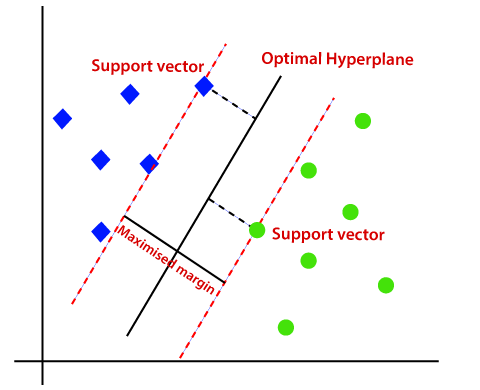
\includegraphics[width=0.5\textwidth]{Images/Chapter1/svm.png}
  \caption{Support Vector Machine (SVM) Decision Boundary Visualization}
  \label{fig:svm}
\end{figure}
The fundamental formula defining the decision boundary of a Support Vector Machine (SVM) is a hyperplane expressed as:
\begin{equation}
  \mathbf{w}^\top \mathbf{x} + b = 0
\end{equation}
where $\mathbf{w}$ is the weight vector normal to the hyperplane, $\mathbf{x}$ is the input feature vector, and $b$ is the bias term.

For binary classification with labels $y_i \in \{+1, -1\}$, the SVM enforces the following constraints on each training point $(\mathbf{x}_i, y_i)$:
\begin{equation}
  y_i \bigl(\mathbf{w}^\top \mathbf{x}_i + b\bigr) \;\ge\; 1,
  \quad \forall\,i.
\end{equation}

The margin width (the distance between the closest points of each class to the hyperplane) is given by $\tfrac{2}{\|\mathbf{w}\|_2}$.  Maximizing this margin is therefore equivalent to minimizing $\|\mathbf{w}\|_2$, leading to the following convex optimization problem:

\begin{align}
  \min_{\mathbf{w},\,b} \quad & \frac{1}{2} \|\mathbf{w}\|_2^2,                             \\
  \text{subject to} \quad     & y_i \bigl(\mathbf{w}^\top \mathbf{x}_i + b\bigr) \;\ge\; 1,
  \quad \forall\,i.
\end{align}
\subsection{Models Training Workflow}
In order to achieve the previous objectives, we followed a step-by-step approach. As shown in Figure~\ref{fig:training}, The training workflow begins with the BraTS dataset. After preprocessing and augmentation, the data is split into training, validation, and test sets. We then train the U-Net segmentation model  in the other hand (separately) we train SVM classifier training, yielding two standalone models for inference that can be combined to form a hybrid model.

\begin{figure}[H]
  \centering
  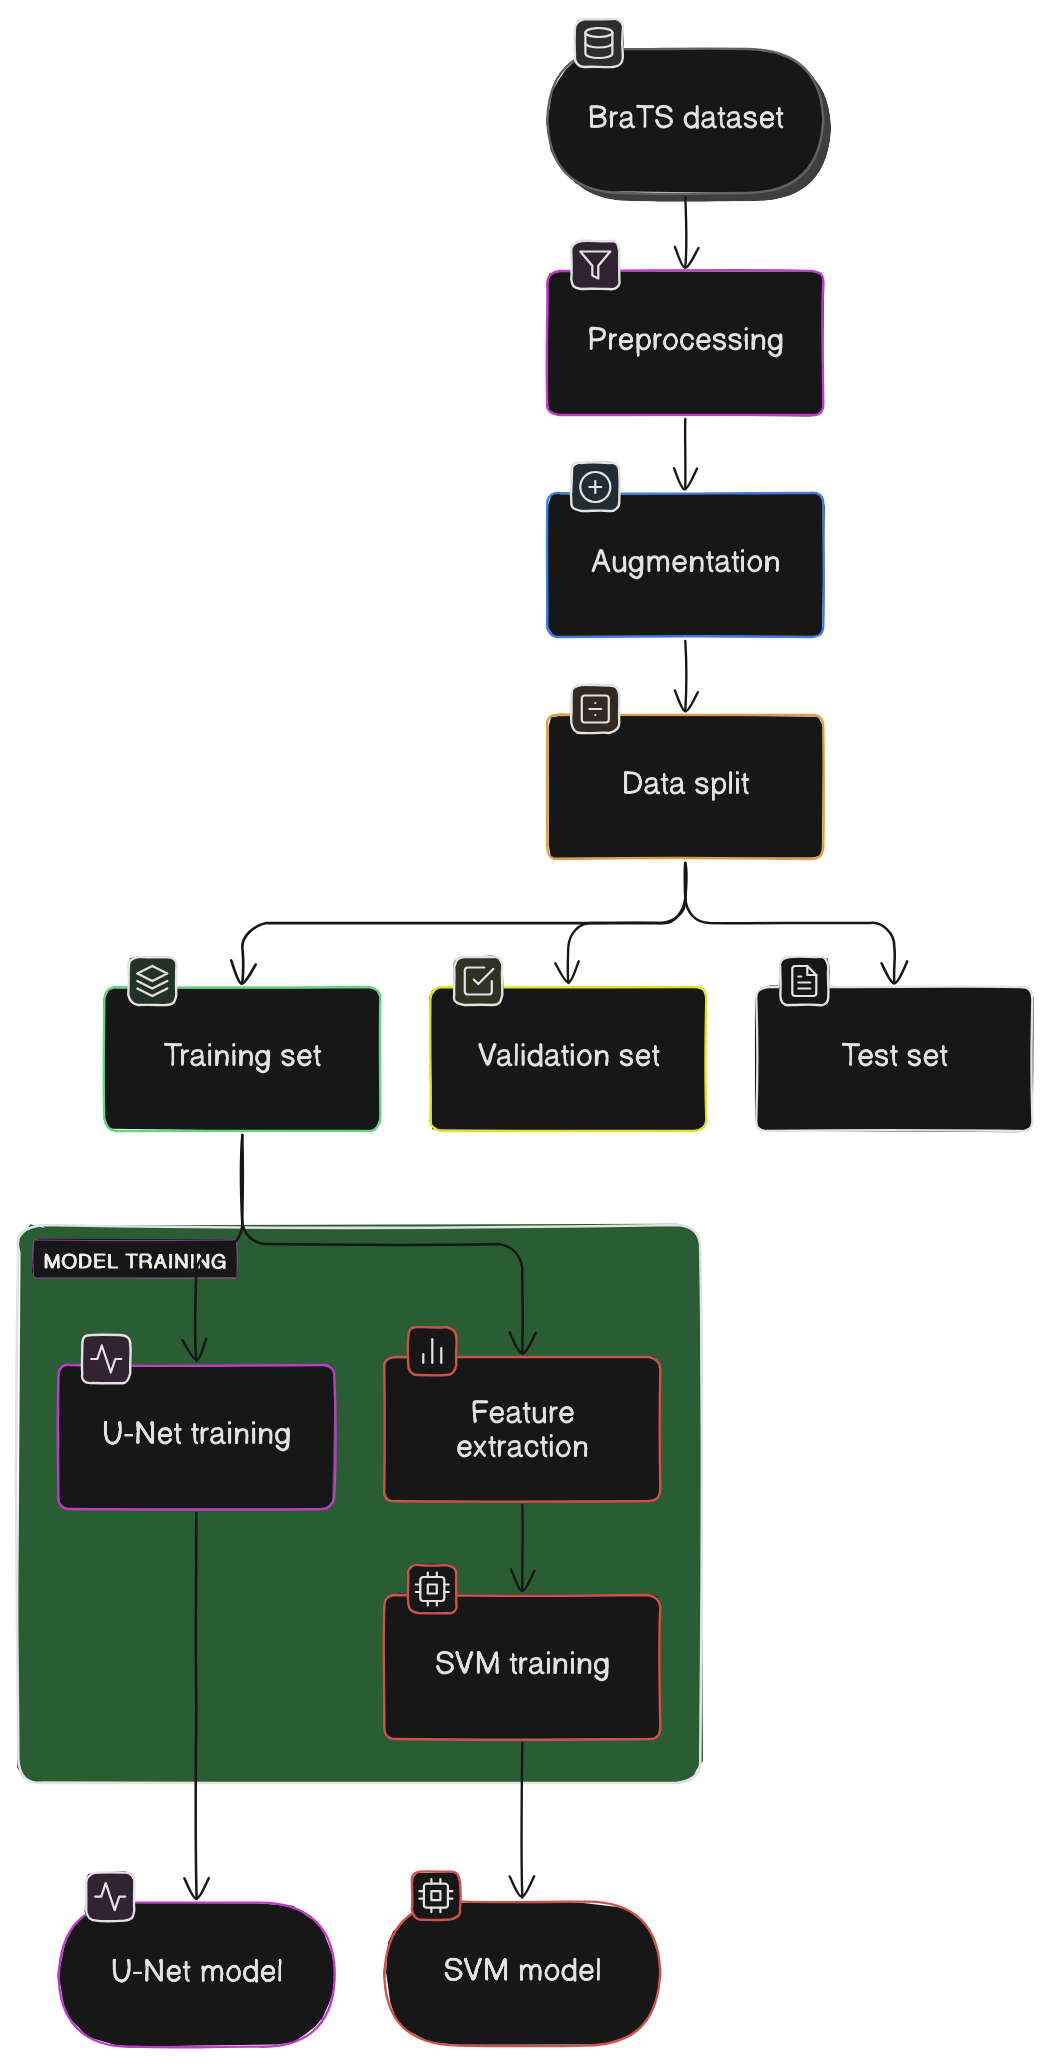
\includegraphics[width=0.6\textwidth]{Images/Chapter3/training.png}
  \caption{Overview of the training workflow.}
  \label{fig:training}
\end{figure}

\section{Dataset and Preprocessing}
\label{sec:contribution-dataset}
In order to train our hybrid model we used the Brain Tumor Segmentation (BraTS) 2020 dataset, which is a collection of multimodal Magnetic Resonance Imaging (MRI) scans used for the segmentation of brain tumors.

\subsection{BraTS Dataset Description}
The dataset includes MRI scans (Figure~\ref{fig:modalities}) from glioma patients, providing four different MRI modalities per patient:
\begin{enumerate}
  \item \textbf{Native (T1)}: Reveals detailed anatomical structures and tissue composition, aiding in the identification of tumors, cysts, and other abnormalities.
  \item \textbf{Post-contrast T1-weighted (T1ce)}: Enhances tumor visibility using a gadolinium-based contrast agent, which accentuates abnormal vascularity and lesion boundaries.
  \item \textbf{T2-weighted (T2)}: Highlights fluid content within brain tissues, which is useful for detecting edema but can sometimes obscure lesions.
  \item \textbf{T2-FLAIR (Fluid Attenuated Inversion Recovery)}: Suppresses the high signal from fluids (e.g., cerebrospinal fluid), making lesions in the white matter more conspicuous.
\end{enumerate}
\begin{figure}[H]
  \centering
  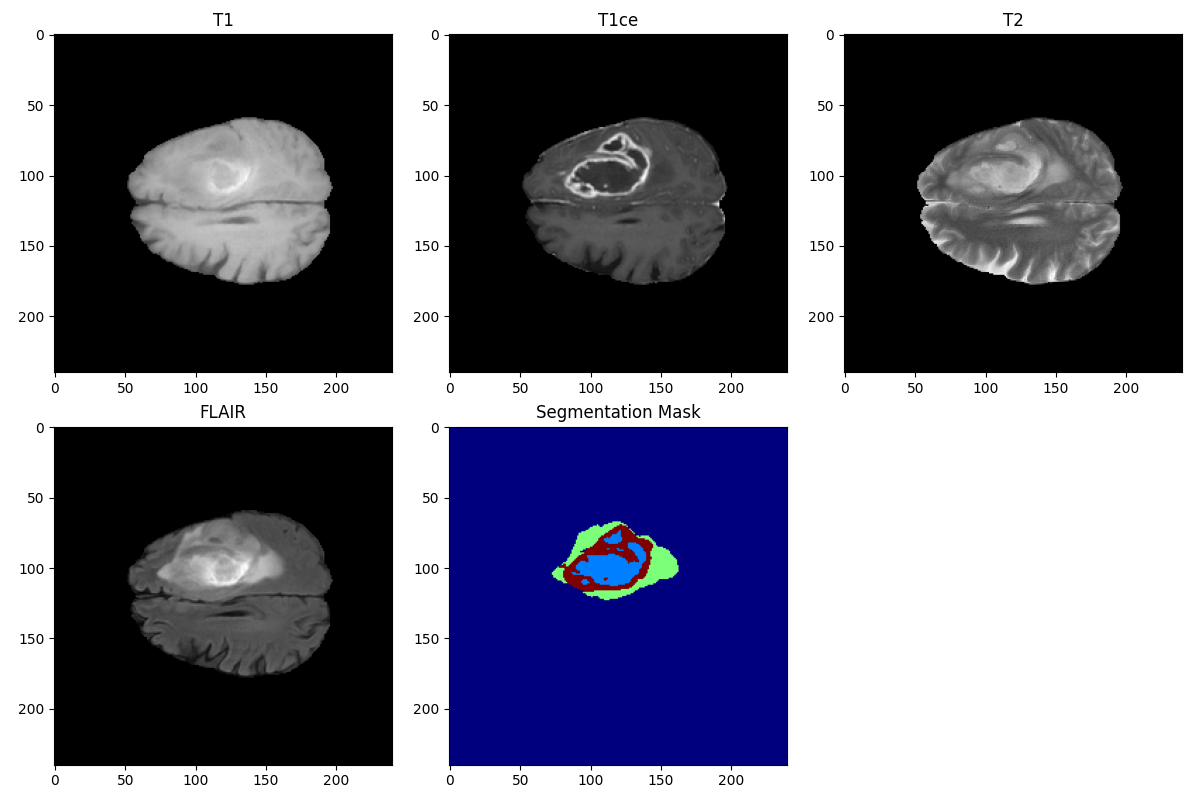
\includegraphics[width=0.8\textwidth]{Images/Chapter3/modalities.png}
  \caption{Brats modalities: T1, T1ce, T2, and T2-FLAIR.}
  \label{fig:modalities}
\end{figure}

These scans (Figure~\ref{fig:modalities}) come with expert-annotated segmentation masks that delineate the tumor into various sub-regions, such as the necrotic and non-enhancing tumor core, the peritumoral edema, and the enhancing tumor. Research has demonstrated that accurate segmentation is linked to improved prognostic assessments and treatment outcomes.

\begin{itemize}
  \item \textbf{Class 0 (Not Tumor):} This class represents normal brain tissue or background, where no tumor tissue is present.
  \item \textbf{Class 1 (Non-Enhancing Tumor):} This class corresponds to the necrotic or non-enhancing core regions of the tumor. These areas typically lack contrast enhancement and may include dead or less active tumor tissue.
  \item \textbf{Class 2 (Edema):} This class identifies regions of peritumoral edema, which is the swelling around the tumor caused by fluid accumulation. Edema is important for understanding the extent of the tumor’s impact on surrounding brain tissue.
  \item \textbf{Class 4 (Enhancing Tumor):} This class captures the actively enhancing parts of the tumor, visible after the administration of a contrast agent. These regions often indicate aggressive tumor tissue with increased blood flow and permeability.
\end{itemize}

To visually interpret these segmentations, we map the categorical labels to a custom colormap. In our example (Figure~\ref{fig:tclass}), we use four distinct colors to represent:

\begin{figure}[H]
  \centering
  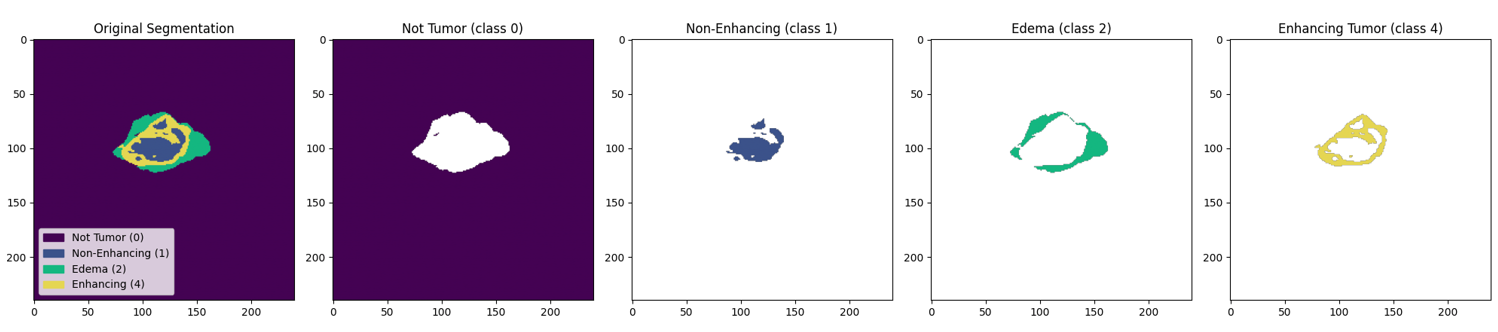
\includegraphics[width=1.1\textwidth]{Images/Chapter3/tclass.png}
  \caption{Segmentation of Tumor classes.}
  \label{fig:tclass}
\end{figure}

\subsection{Dataset Splitting}
To train and evaluate our model effectively, we need to partition our dataset into three subsets:
\begin{itemize}
  \item \textbf{Training Set (70\%):} Used to learn the model parameters.
  \item \textbf{Validation Set (approximately 20\%):} Used for tuning hyperparameters and preventing overfitting.
  \item \textbf{Test Set (10\%):} Used for assessing the final model’s performance on unseen data.
\end{itemize}
This split can be done randomly or in a stratified manner (to preserve the class distribution), which is especially useful when dealing with imbalanced datasets. Properly splitting the dataset is crucial for building a robust model that generalizes well to new data.
\begin{figure}[H]
  \centering
  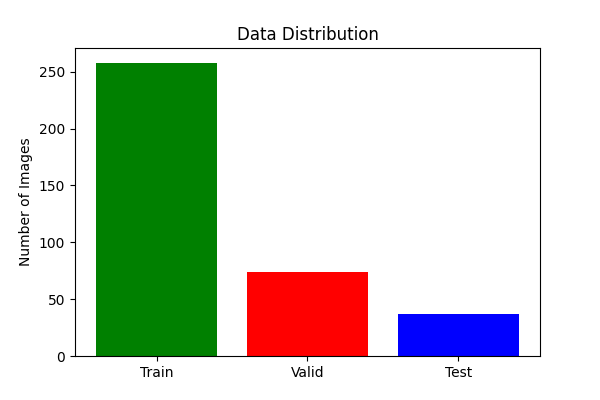
\includegraphics[width=0.8\textwidth]{Images/Chapter3/data_distribution.png}
  \caption{Dataset splitting: training, validation, and test sets.}
  \label{fig:data_distribution}
\end{figure}


\subsection{Data Preprocessing}
\label{sec:contribution-preprocessing}

Before feeding MR volumes into our models, we apply a series of standardized preprocessing steps to ensure consistency and improve model robustness. Our pipeline operates on 2D axial slices extracted from 3D volumes, as follows:

\begin{enumerate}
  \item \textbf{Slice Extraction.}
        For each patient volume, we select 100 consecutive axial slices starting at index 22. This avoids initial and final slices that contain little anatomical information.

  \item \textbf{Resizing.}
        \begin{itemize}
          \item \emph{Image Slices:} Each extracted slice is resized to \texttt{128$\times$128} pixels to match the U-Net input dimensions.
          \item \emph{Segmentation Masks:} Corresponding ground-truth masks are first resized to \texttt{240$\times$240} (to preserve label fidelity) and later downsampled alongside images during one-hot encoding.
        \end{itemize}

  \item \textbf{Intensity Normalization.}
        All pixel intensities in a slice are divided by the global maximum value of that volume, scaling inputs to the \([0,1]\) range. This step harmonizes contrast across patients and modalities.

  \item \textbf{Augmentation.}
        To increase effective training diversity, random geometric transformations are applied during batch generation:
        \begin{itemize}
          \item Horizontal and vertical flips (each with 50\% probability).
          \item Rotations by multiples of 90° (randomly chosen among 0°, 90°, 180°, 270°).
        \end{itemize}
\end{enumerate}


\section{Evaluation Metrics}
\label{sec:evaluation-metrics}

To quantify the performance of our segmentation and classification models, we use a suite of metrics that assess accuracy, robustness, and specificity:

\begin{itemize}
  \item \textbf{Accuracy}
        \[
          \text{Accuracy} \;=\; \frac{\text{TP} + \text{TN}}{\text{TP} + \text{TN} + \text{FP} + \text{FN}}
        \]
        \begin{itemize}
          \item \emph{Segmentation:} Proportion of correctly classified pixels (tumor vs.\ non‐tumor).
          \item \emph{Classification:} Proportion of correctly classified patients (LGG vs.\ HGG).
        \end{itemize}

  \item \textbf{Precision} (Positive Predictive Value)
        \[
          \text{Precision} \;=\; \frac{\text{TP}}{\text{TP} + \text{FP}}
        \]
        \begin{itemize}
          \item \emph{Segmentation:} Fraction of predicted tumor pixels that are actually tumor.
          \item \emph{Classification:} Fraction of patients predicted as HGG who truly have HGG.
        \end{itemize}

  \item \textbf{Recall} (Sensitivity or True Positive Rate)
        \[
          \text{Recall} \;=\; \frac{\text{TP}}{\text{TP} + \text{FN}}
        \]
        \begin{itemize}
          \item \emph{Segmentation:} Fraction of actual tumor pixels correctly identified.
          \item \emph{Classification:} Fraction of actual HGG patients correctly identified.
        \end{itemize}

  \item \textbf{Specificity} (True Negative Rate)
        \[
          \text{Specificity} \;=\; \frac{\text{TN}}{\text{TN} + \text{FP}}
        \]
        \begin{itemize}
          \item \emph{Segmentation:} Fraction of non‐tumor pixels correctly classified as non‐tumor.
          \item \emph{Classification:} Fraction of actual LGG patients correctly identified as LGG.
        \end{itemize}

  \item \textbf{F1‐Score}
        \[
          \text{F1} \;=\; \frac{2\,\text{TP}}{2\,\text{TP} + \text{FP} + \text{FN}}
        \]
        \begin{itemize}
          \item \emph{Classification:} Harmonic mean of precision and recall for each class, then averaged.
        \end{itemize}

  \item \textbf{Intersection over Union (IoU)}
        Also called Jaccard index:
        \[
          \text{IoU} \;=\; \frac{\text{TP}}{\text{TP} + \text{FP} + \text{FN}}
        \]
        \begin{itemize}
          \item \emph{Segmentation:} Overlap between predicted and ground‐truth tumor masks, averaged over classes (mIoU).
        \end{itemize}

  \item \textbf{Dice Coefficient} (Segmentation F1)
        \[
          \text{Dice} \;=\; \frac{2\,\text{TP}}{2\,\text{TP} + \text{FP} + \text{FN}}
        \]
        \begin{itemize}
          \item \emph{Segmentation:} Emphasizes overlap; computed overall and per‐class (necrotic, edema, enhancing).
        \end{itemize}

  \item \textbf{Confusion Matrix}
        A contingency table of true vs.\ predicted labels:
        \[
          \begin{array}{c|cc}
                                   & \text{Predicted Positive} & \text{Predicted Negative} \\ \hline
            \text{Actual Positive} & \text{TP}                 & \text{FN}                 \\
            \text{Actual Negative} & \text{FP}                 & \text{TN}                 \\
          \end{array}
        \]
        \begin{itemize}
          \item \emph{Classification:} Provides counts of TP, FP, FN, TN for LGG/HGG.
        \end{itemize}

  \item \textbf{ROC AUC} (Area Under the Receiver Operating Characteristic Curve)
        \[
          \text{AUC} \;=\; \frac{1}{2} \sum_{i=1}^{n} (\text{TPR}_{i} + \text{TPR}_{i-1}) \times (\text{FPR}_{i} - \text{FPR}_{i-1})
        \]

        \begin{itemize}
          \item \emph{Classification:} Measures the trade‐off between sensitivity and specificity across thresholds.
        \end{itemize}
        \paragraph{knowing that:}
        \begin{itemize}
          \item \(\text{TP}\) = number of true positive cases (correctly predicted positive).
          \item \(\text{TN}\) = number of true negative cases (correctly predicted negative).
          \item \(\text{FP}\) = number of false positive cases (incorrectly predicted positive).
          \item \(\text{FN}\) = number of false negative cases (incorrectly predicted negative).
          \item \(\text{TPR}\) = true positive rate (recall): \(\text{TPR} = \frac{\text{TP}}{\text{TP} + \text{FN}}\).
          \item \(\text{FPR}\) = false positive rate: \(\text{FPR} = \frac{\text{FP}}{\text{FP} + \text{TN}}\).
          \item \(\text{TNR}\) = true negative rate (specificity): \(\text{TNR} = \frac{\text{TN}}{\text{TN} + \text{FP}}\).
          \item \(\text{FNR}\) = false negative rate: \(\text{FNR} = \frac{\text{FN}}{\text{FN} + \text{TP}}\).
        \end{itemize}

\end{itemize}




\section{Results and Discussion}
\subsection{Segmentation Results}
\label{sec:segmentation-results}
In this section, we present the results of our U-Net segmentation model on the BraTS2020 dataset. The model was trained for 50 epochs with a batch size of 16, we will discuss the end results of the training and validation process, including loss and accuracy metrics.

\subsubsection{Accuracy}
The model achieved a pixel-level accuracy of 99.3\%, demonstrating that the vast majority of pixels were correctly classified. The accuracy trend, illustrated in Figure~\ref{fig:unet-acc}, confirms stable and effective learning throughout the training process.
\begin{figure}[ht]
  \centering
  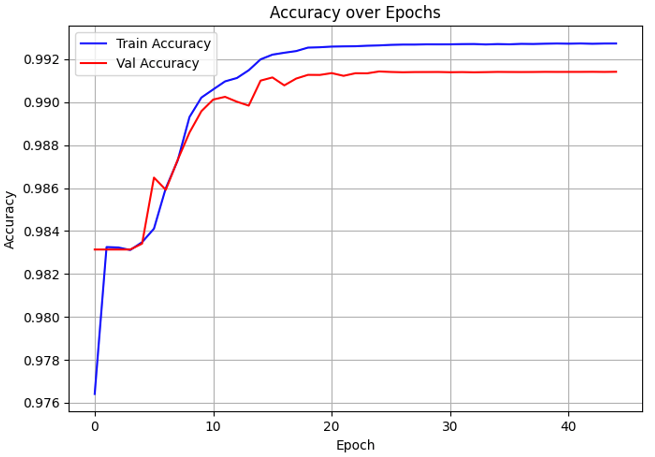
\includegraphics[width=0.6\textwidth]{Images/Chapter3/unet_acc.png}
  \caption{Training and Validation Accuracy over Epochs for the U-Net Segmentation Model}
  \label{fig:unet-acc}
\end{figure}

\subsubsection{Loss}
A final loss value of 0.0231 indicates a strong alignment between predictions and ground truth. As shown in Figure~\ref{fig:unet-loss}, the training and validation loss curves demonstrate smooth convergence, reflecting effective learning and minimal overfitting.

\begin{figure}[h]
  \centering
  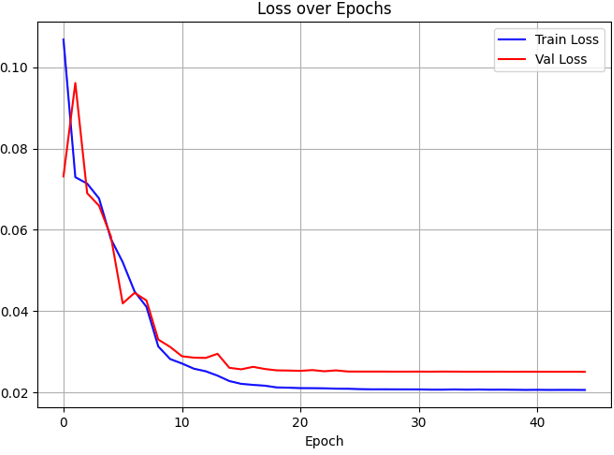
\includegraphics[width=0.6\textwidth]{Images/Chapter3/unet_loss.png}
  \caption{Training and Validation Loss over Epochs for the U-Net Segmentation Model}
  \label{fig:unet-loss}
\end{figure}


\subsubsection{Dice Coefficient}
The model achieved an overall Dice score of 58.98\%, indicating a reasonable level of agreement between the predicted and ground truth tumor regions. Additionally, per-class Dice scores were computed to assess performance across specific tumor subregions. Figure~\ref{fig:unet-dice} illustrates the training and validation Dice coefficient trends throughout the learning process.
\begin{figure}[h]
  \centering
  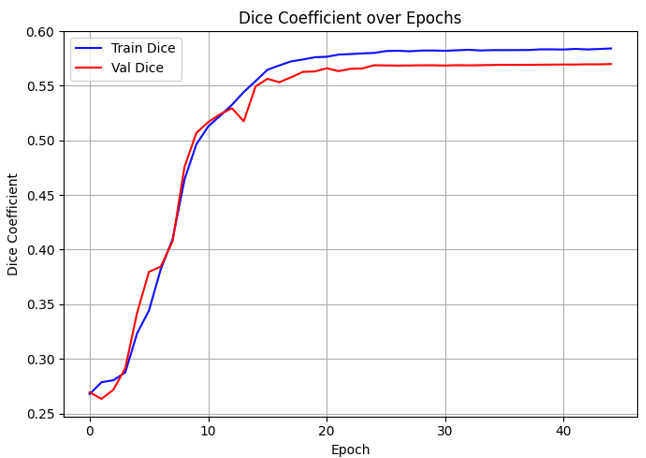
\includegraphics[width=0.6\textwidth]{Images/Chapter3/unet_dice.png}
  \caption{Training and Validation Dice Coefficient over Epochs for the U-Net Segmentation Model}
  \label{fig:unet-dice}
\end{figure}


\subsubsection{Mean IoU}
The model achieved a mean Intersection over Union (\glsxtrshort{iou}) of 74.66\%, reflecting a solid overlap between predicted and actual segmentation masks. Figure~\ref{fig:unet-iou} illustrates the progression of training and validation IoU values, confirming consistent performance across classes.
\begin{figure}[h]
  \centering
  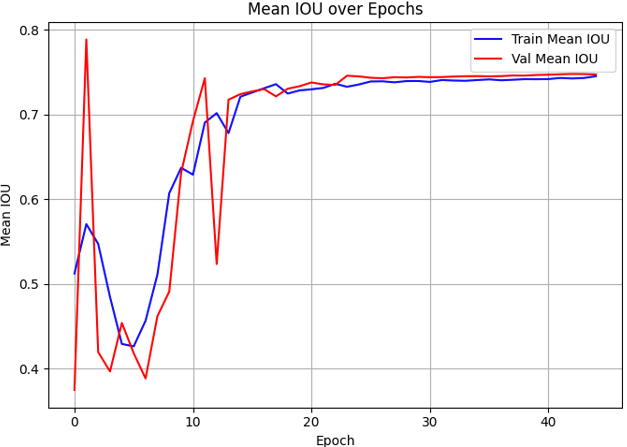
\includegraphics[width=0.6\textwidth]{Images/Chapter3/unet_iou.png}
  \caption{Training and Validation Mean IoU over Epochs for the U-Net Segmentation Model}
  \label{fig:unet-iou}
\end{figure}
\begin{table}[ht]
  \centering
  \caption{Performance Metrics for the U-Net Segmentation Model}
  \label{tab:segmentation-results}
  \begin{tabular}{l r}
    \hline
    \textbf{Metric}  & \textbf{Value} \\
    \hline
    Loss             & 0.0231         \\
    Accuracy         & 99.30\,\%      \\
    Mean IoU         & 74.66\,\%      \\
    Dice Coefficient & 58.98\,\%      \\
    Precision        & 99.37\,\%      \\
    Sensitivity      & 99.08\,\%      \\
    Specificity      & 99.79\,\%      \\
    \hline
  \end{tabular}
\end{table}

\begin{figure}[h]
  \centering
  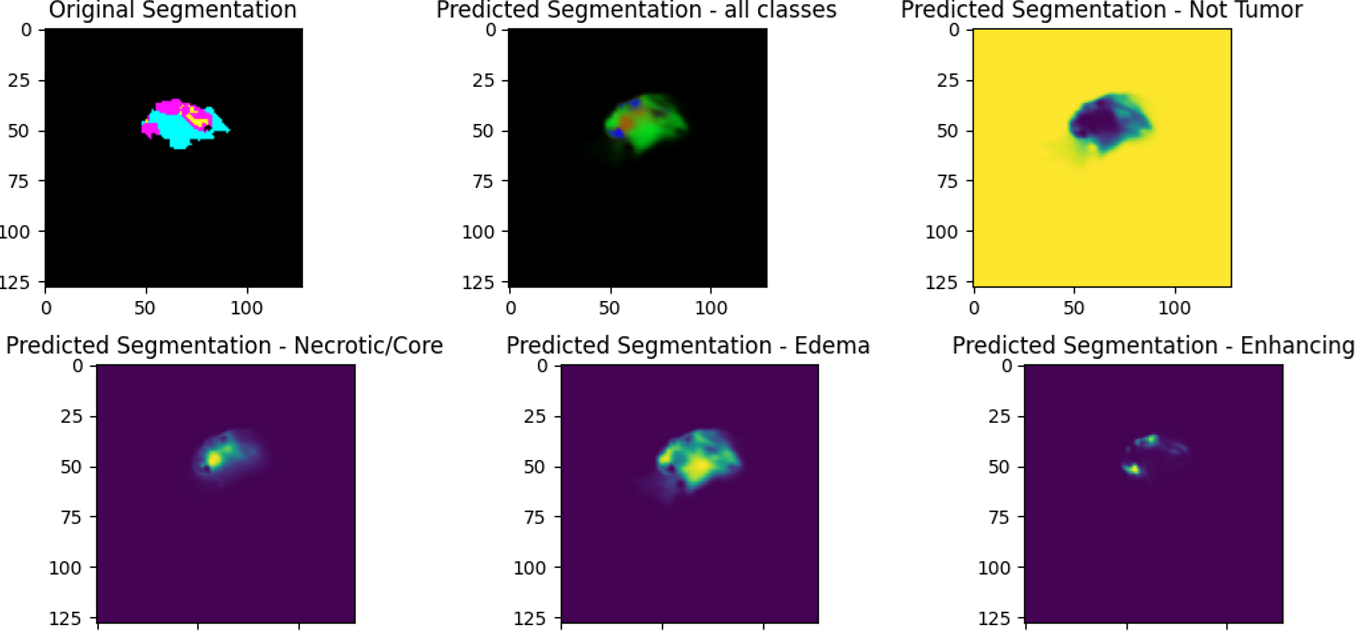
\includegraphics[width=0.9\textwidth]{Images/Chapter3/seg.png}
  \caption{Sample of a Predicted tumor segmentation masks.}
  \label{fig:segmentation-example}
\end{figure}

\newpage\
\subsection{Classification Results}
\label{sec:classification-results}

Table~\ref{tab:svm-report} summarizes the classification performance of the Support Vector Machine (SVM) model on the held-out test set. The model achieved an overall accuracy of 93.24\,\%, indicating strong generalization. High-grade gliomas (HGG) were classified with high precision (95\,\%) and recall (97\,\%), resulting in an F1-score of 96\,\%. In contrast, low-grade gliomas (LGG) achieved slightly lower metrics, with an F1-score of 83\,\%, reflecting a minor challenge in capturing the more subtle features associated with LGG.

The macro average shows a balanced view of precision and recall across both classes, with scores around 88–90\,\%, while the weighted average—which takes class support into account—remains consistent at 93\,\%. These results confirm the SVM model's reliability and effectiveness in brain tumor grade classification, particularly in detecting HGG, which typically has more distinct patterns and features.

\begin{table}[ht]
  \centering
  \caption{Performance Metrics of SVM Classifier on the Test Set}
  \label{tab:svm-report}
  \begin{tabular}{lcccc}
    \hline
    Class        & Precision                     & Recall & F1-Score & Support \\
    \hline
    LGG (0)      & 86\,\%                        & 80\,\% & 83\,\%   & 15      \\
    HGG (1)      & 95\,\%                        & 97\,\% & 96\,\%   & 59      \\
    \hline
    Accuracy     & \multicolumn{4}{c}{93.24\,\%}                               \\
    Macro avg    & 90\,\%                        & 88\,\% & 89\,\%   & 74      \\
    Weighted avg & 93\,\%                        & 93\,\% & 93\,\%   & 74      \\
    \hline
  \end{tabular}
\end{table}

\begin{figure}[H]
  \centering
  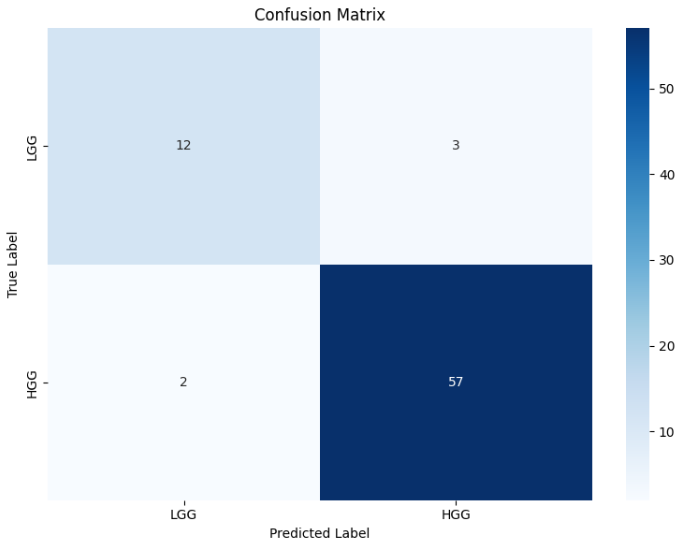
\includegraphics[width=0.6\textwidth]{Images/Chapter3/confusion.png}
  \caption{Confusion matrix for the SVM classifier.}
  \label{fig:confusion}
\end{figure}


\section{Application Demo}
\label{sec:contribution-demo}

To illustrate end‐user interaction, we developed a lightweight demo application that integrates our trained U-Net and SVM models into a single GUI. The application  consists of two main pages:

\subsection{Upload Page}
\label{sec:contribution-demo-upload}

Presents an HTML form where the user can select and upload a brain tumor image (2D slice).
Upon submission, the form sends a POST request to the \texttt{/results} route.

\begin{figure}[H]
  \centering
  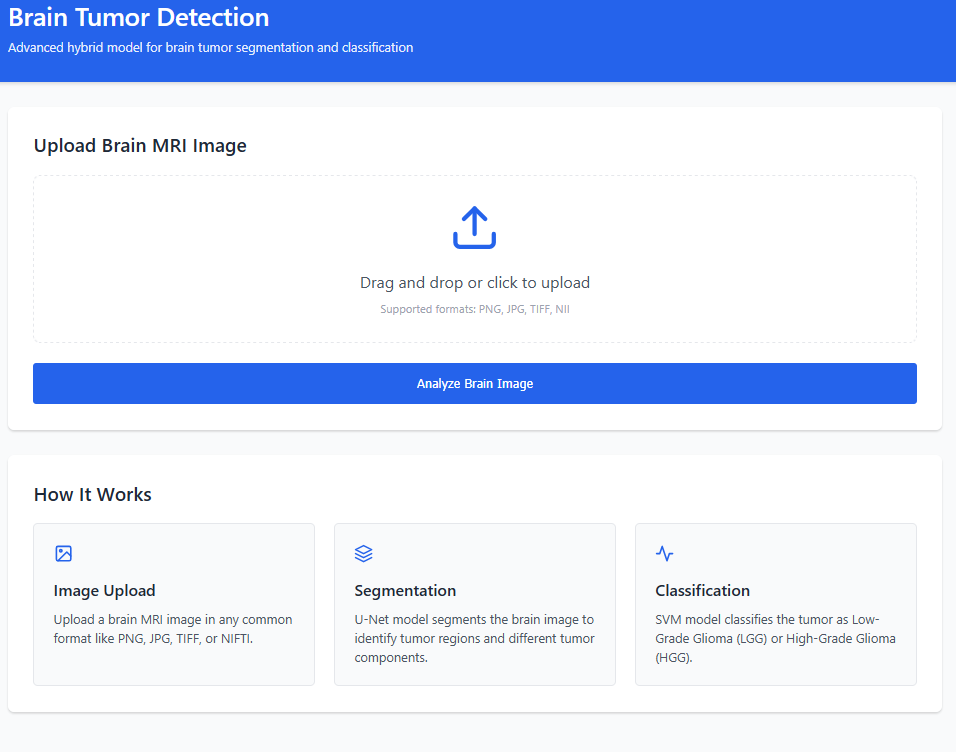
\includegraphics[width=1\textwidth]{Images/Chapter3/app_interface.png}
  \caption{Upload page of the application demo.}
  \label{fig:demo-upload}
\end{figure}

\subsection{Results Page}
\label{sec:contribution-demo-results}

Receives the uploaded image, runs the preprocessing, segmentation (U-Net), feature extraction, and classification (SVM) pipeline, and then renders:
\begin{itemize}
  \item The original input image.
  \item The segmentation mask overlaid on the input.
  \item The predicted tumor grade (LGG/HGG) with its confidence score.
\end{itemize}
\begin{figure}[H]
  \centering
  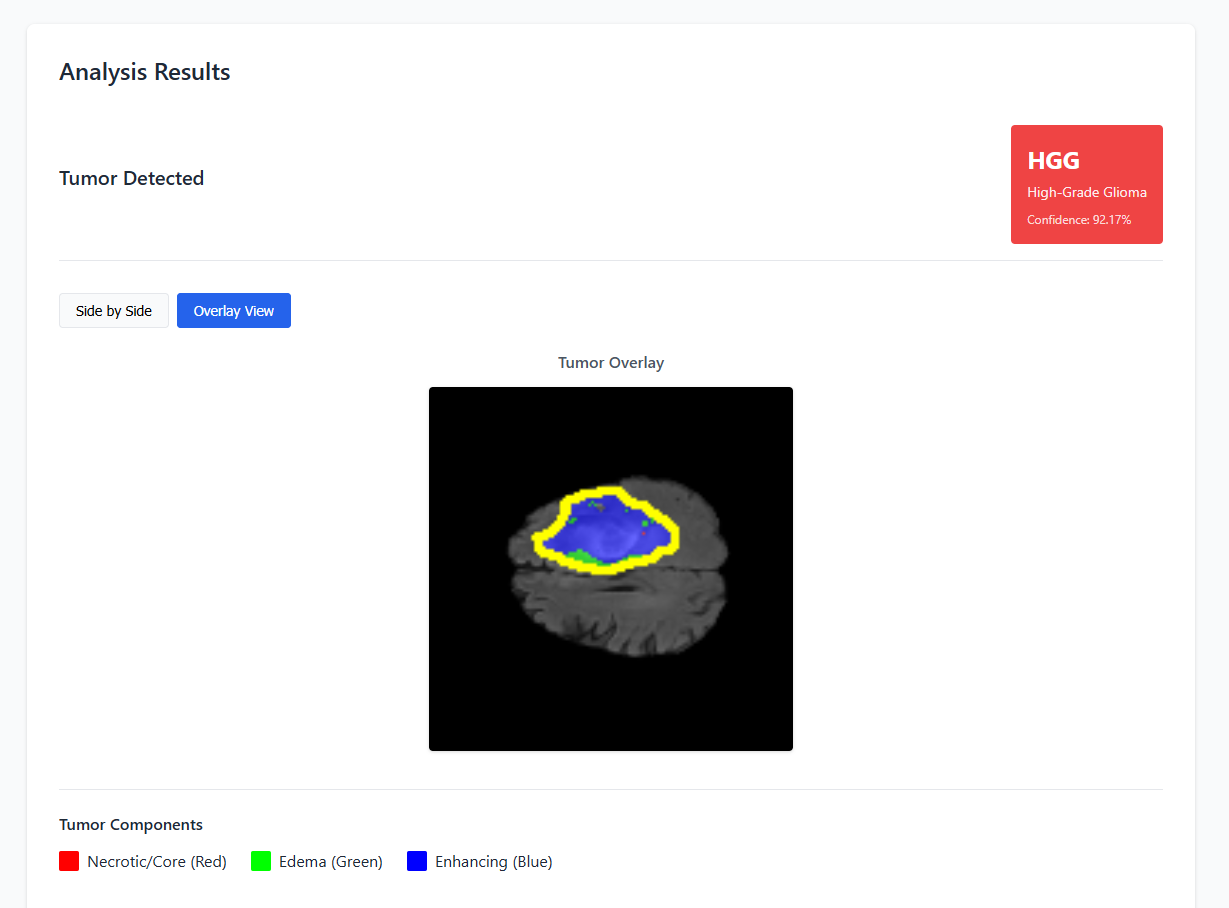
\includegraphics[width=1\textwidth]{Images/Chapter3/app_result.png}
  \caption{Results page of the application demo.}
  \label{fig:demo-results}
\end{figure}

\section{Conclusion}
\label{sec:contribution-conclusion}

In this chapter, we have presented a comprehensive methodology for automated brain tumor detection and classification using MR images. Our approach integrates a U-Net-based segmentation model with an SVM classifier, achieving high accuracy and robust performance across multiple evaluation metrics. The segmentation module demonstrated reliable delineation of tumor subregions, while the classification module effectively distinguished between high-grade and low-grade gliomas. Additionally, we showcased the practical application of our framework through a user-friendly demo application, highlighting its potential for real-world clinical use. These contributions underscore the effectiveness of combining deep learning and classical machine learning techniques in addressing complex medical imaging challenges. Future work could explore further optimization of the pipeline, incorporation of additional data modalities, and validation on larger, more diverse datasets.




\chapter{Conclusion générale (2 pages max)}

\section{Contributions}
Insérez un texte décrivant les contributions de votre projet. 

\section{Critique du travail}
Insérez un texte faisant une critique du travail.  

\section{Travaux futurs et perspectives}
Insérez un texte décrivant les extensions possibles du travail et les perspectives. 


\addcontentsline{toc}{chapter}{bibliography}
\bibliographystyle{IEEEtranN}
\bibliography{bibliography}


\appendix

% \chapter{Titre de l’annexe ici}

\section{}


\subsection{}
% \chapter{Titre de l’annexe ici}

\section{}

\subsection{}


\end{document}
